% Options for packages loaded elsewhere
\PassOptionsToPackage{unicode}{hyperref}
\PassOptionsToPackage{hyphens}{url}
%
\documentclass[
  letterpaper,
  DIV=11,
  numbers=noendperiod]{scrartcl}

\usepackage{amsmath,amssymb}
\usepackage{iftex}
\ifPDFTeX
  \usepackage[T1]{fontenc}
  \usepackage[utf8]{inputenc}
  \usepackage{textcomp} % provide euro and other symbols
\else % if luatex or xetex
  \usepackage{unicode-math}
  \defaultfontfeatures{Scale=MatchLowercase}
  \defaultfontfeatures[\rmfamily]{Ligatures=TeX,Scale=1}
\fi
\usepackage{lmodern}
\ifPDFTeX\else  
    % xetex/luatex font selection
\fi
% Use upquote if available, for straight quotes in verbatim environments
\IfFileExists{upquote.sty}{\usepackage{upquote}}{}
\IfFileExists{microtype.sty}{% use microtype if available
  \usepackage[]{microtype}
  \UseMicrotypeSet[protrusion]{basicmath} % disable protrusion for tt fonts
}{}
\makeatletter
\@ifundefined{KOMAClassName}{% if non-KOMA class
  \IfFileExists{parskip.sty}{%
    \usepackage{parskip}
  }{% else
    \setlength{\parindent}{0pt}
    \setlength{\parskip}{6pt plus 2pt minus 1pt}}
}{% if KOMA class
  \KOMAoptions{parskip=half}}
\makeatother
\usepackage{xcolor}
\setlength{\emergencystretch}{3em} % prevent overfull lines
\setcounter{secnumdepth}{5}
% Make \paragraph and \subparagraph free-standing
\makeatletter
\ifx\paragraph\undefined\else
  \let\oldparagraph\paragraph
  \renewcommand{\paragraph}{
    \@ifstar
      \xxxParagraphStar
      \xxxParagraphNoStar
  }
  \newcommand{\xxxParagraphStar}[1]{\oldparagraph*{#1}\mbox{}}
  \newcommand{\xxxParagraphNoStar}[1]{\oldparagraph{#1}\mbox{}}
\fi
\ifx\subparagraph\undefined\else
  \let\oldsubparagraph\subparagraph
  \renewcommand{\subparagraph}{
    \@ifstar
      \xxxSubParagraphStar
      \xxxSubParagraphNoStar
  }
  \newcommand{\xxxSubParagraphStar}[1]{\oldsubparagraph*{#1}\mbox{}}
  \newcommand{\xxxSubParagraphNoStar}[1]{\oldsubparagraph{#1}\mbox{}}
\fi
\makeatother


\providecommand{\tightlist}{%
  \setlength{\itemsep}{0pt}\setlength{\parskip}{0pt}}\usepackage{longtable,booktabs,array}
\usepackage{calc} % for calculating minipage widths
% Correct order of tables after \paragraph or \subparagraph
\usepackage{etoolbox}
\makeatletter
\patchcmd\longtable{\par}{\if@noskipsec\mbox{}\fi\par}{}{}
\makeatother
% Allow footnotes in longtable head/foot
\IfFileExists{footnotehyper.sty}{\usepackage{footnotehyper}}{\usepackage{footnote}}
\makesavenoteenv{longtable}
\usepackage{graphicx}
\makeatletter
\def\maxwidth{\ifdim\Gin@nat@width>\linewidth\linewidth\else\Gin@nat@width\fi}
\def\maxheight{\ifdim\Gin@nat@height>\textheight\textheight\else\Gin@nat@height\fi}
\makeatother
% Scale images if necessary, so that they will not overflow the page
% margins by default, and it is still possible to overwrite the defaults
% using explicit options in \includegraphics[width, height, ...]{}
\setkeys{Gin}{width=\maxwidth,height=\maxheight,keepaspectratio}
% Set default figure placement to htbp
\makeatletter
\def\fps@figure{htbp}
\makeatother
% definitions for citeproc citations
\NewDocumentCommand\citeproctext{}{}
\NewDocumentCommand\citeproc{mm}{%
  \begingroup\def\citeproctext{#2}\cite{#1}\endgroup}
\makeatletter
 % allow citations to break across lines
 \let\@cite@ofmt\@firstofone
 % avoid brackets around text for \cite:
 \def\@biblabel#1{}
 \def\@cite#1#2{{#1\if@tempswa , #2\fi}}
\makeatother
\newlength{\cslhangindent}
\setlength{\cslhangindent}{1.5em}
\newlength{\csllabelwidth}
\setlength{\csllabelwidth}{3em}
\newenvironment{CSLReferences}[2] % #1 hanging-indent, #2 entry-spacing
 {\begin{list}{}{%
  \setlength{\itemindent}{0pt}
  \setlength{\leftmargin}{0pt}
  \setlength{\parsep}{0pt}
  % turn on hanging indent if param 1 is 1
  \ifodd #1
   \setlength{\leftmargin}{\cslhangindent}
   \setlength{\itemindent}{-1\cslhangindent}
  \fi
  % set entry spacing
  \setlength{\itemsep}{#2\baselineskip}}}
 {\end{list}}
\usepackage{calc}
\newcommand{\CSLBlock}[1]{\hfill\break\parbox[t]{\linewidth}{\strut\ignorespaces#1\strut}}
\newcommand{\CSLLeftMargin}[1]{\parbox[t]{\csllabelwidth}{\strut#1\strut}}
\newcommand{\CSLRightInline}[1]{\parbox[t]{\linewidth - \csllabelwidth}{\strut#1\strut}}
\newcommand{\CSLIndent}[1]{\hspace{\cslhangindent}#1}

\usepackage{booktabs}
\usepackage{caption}
\usepackage{longtable}
\usepackage{colortbl}
\usepackage{array}
\usepackage{anyfontsize}
\usepackage{multirow}
\KOMAoption{captions}{tableheading}
\usepackage[left]{lineno}
\linenumbers
\usepackage{xcolor}
\usepackage{float}
\floatplacement{table}{H}
\usepackage{setspace}
\makeatletter
\@ifpackageloaded{caption}{}{\usepackage{caption}}
\AtBeginDocument{%
\ifdefined\contentsname
  \renewcommand*\contentsname{Table of contents}
\else
  \newcommand\contentsname{Table of contents}
\fi
\ifdefined\listfigurename
  \renewcommand*\listfigurename{List of Figures}
\else
  \newcommand\listfigurename{List of Figures}
\fi
\ifdefined\listtablename
  \renewcommand*\listtablename{List of Tables}
\else
  \newcommand\listtablename{List of Tables}
\fi
\ifdefined\figurename
  \renewcommand*\figurename{Figure}
\else
  \newcommand\figurename{Figure}
\fi
\ifdefined\tablename
  \renewcommand*\tablename{Table}
\else
  \newcommand\tablename{Table}
\fi
}
\@ifpackageloaded{float}{}{\usepackage{float}}
\floatstyle{ruled}
\@ifundefined{c@chapter}{\newfloat{codelisting}{h}{lop}}{\newfloat{codelisting}{h}{lop}[chapter]}
\floatname{codelisting}{Listing}
\newcommand*\listoflistings{\listof{codelisting}{List of Listings}}
\makeatother
\makeatletter
\makeatother
\makeatletter
\@ifpackageloaded{caption}{}{\usepackage{caption}}
\@ifpackageloaded{subcaption}{}{\usepackage{subcaption}}
\makeatother

\ifLuaTeX
  \usepackage{selnolig}  % disable illegal ligatures
\fi
\usepackage{bookmark}

\IfFileExists{xurl.sty}{\usepackage{xurl}}{} % add URL line breaks if available
\urlstyle{same} % disable monospaced font for URLs
\hypersetup{
  pdftitle={Snow Interception Relationships with Meteorology and Canopy Density in a Subalpine Forest},
  hidelinks,
  pdfcreator={LaTeX via pandoc}}


\title{Snow Interception Relationships with Meteorology and Canopy
Density in a Subalpine Forest}
\author{}
\date{}

\begin{document}
\maketitle


\setstretch{1.5}

\textbf{Authors:}

Alexander Charles Cebulski\textsuperscript{1} (ORCID ID -
0000-0001-7910-5056)

John Willard Pomeroy\textsuperscript{1} (ORCID ID - 0000-0002-4782-7457)

\textsuperscript{1}Centre for Hydrology, University of Saskatchewan,
Canmore, Canada

\textbf{Corresponding Author:} A.C. Cebulski, 50 Lincoln Park, Canmore,
Alberta, Canada, T1W 3E9, alex.cebulski@usask.ca

\textbf{Abstract:} Snow accumulation models differ in how snow
interception and ablation processes are represented and thus their
application to diverse climates and forest types is uncertain. Existing
parameterizations of initial snow interception before unloading include
inherently coupled canopy snow accumulation and ablation processes. This
leads to difficulty in diagnosing processes and adding possible errors
to simulations when incorporated as canopy interception routines in
models that already account for canopy snow ablation. This study
evaluates the theory underpinning parameterizations of initial snow
interception using high-temporal resolution and fine-scale measurements
of throughfall for events with minimal snow ablation and redistribution
in both the canopy and on the ground. The relationship between these
throughfall measurements, event meteorology, and a novel lidar-based
canopy density measurement are assessed in two subalpine forest plots in
the Canadian Rockies. Contrary to existing theories, no association of
canopy snow load or air temperature with interception efficiency was
observed. Instead, canopy density emerged as the primary factor
governing snow accumulation. A wind-driven snowfall event demonstrated
that non-vertical hydrometeor trajectories can significantly increase
snow-leaf contact area, thereby enhancing initial interception before
ablation. Prediction of interception efficiency for this event improved
dramatically when adjusted for hydrometeor trajectory angle based on a
wind speed at one-third of the canopy height. Snow-leaf contact area
showed a high sensitivity to wind speed, increasing by up to 95\% with a
1 m s\textsuperscript{-1} wind speed. The study proposes a new
parameterization that calculates throughfall, independent of processes
that ablate snow from the canopy, as a function of snowfall, canopy
cover, and above canopy wind speed. This new parameterization
successfully estimated subcanopy snow accumulation for a snowfall event
at two forest plots measured using lidar and snow surveys. By separating
canopy snow ablation from snow interception processes, this new model
offers potentially improved prediction of subcanopy snow accumulation
when combined with canopy snow ablation parameterizations.

\textbf{Keywords:} snow interception, throughfall, ablation, forest,
snowpack, lidar, process-based modelling

\section{Introduction}\label{introduction}

Over half of North America's snow-covered zone is covered by forests
(Kim et al., 2017), significantly impacting the accumulation and
redistribution of snowpacks and subsequent snowmelt runoff. Essery et
al. (2003) estimated that 25--45\% of annual snowfall may be lost to the
atmosphere due to sublimation of snow intercepted in forest canopies
globally. Snow intercepted in the canopy can sublimate and melt at much
higher rates than the subcanopy snowpack (Katsushima et al., 2023;
Lundberg \& Hallidin, 1994; Pomeroy et al., 1998), reducing the amount
of snow available for runoff. Vegetation structure is one of the primary
factors controlling the partitioning of snowfall into throughfall and
interception (Hedstrom \& Pomeroy, 1998; Storck et al., 2002), and thus
governs the quantity of snow subject to sublimation from the canopy.
However, forest thinning efforts aimed at limiting sublimation losses to
increase snowmelt runoff do not always lead to a corresponding increase
in spring streamflow (Golding \& Swanson, 1978; Harpold et al., 2020;
Pomeroy et al., 2012; Troendle, 1983). This may be due to increased
ablation rates when forest cover is reduced, desynchronization of
snowmelt, and sub-surface hydrology interactions (Ellis et al., 2013;
Musselman et al., 2015; Pomeroy et al., 1997; Safa et al., 2021; Varhola
et al., 2010). Given the significant impact of forest cover on
snowpacks, along with the limited or absent monitoring networks for
subcanopy snow accumulation (Rittger et al., 2020; Vionnet et al.,
2021), land management, ecological conservation, and water resource
decisions depend on reliable models of snow redistribution.

Hedstrom \& Pomeroy (1998), working in the cold continental boreal
forest, proposed that initial snow interception efficiency was
controlled by the maximum canopy load which itself was a function of
leaf area index and new snow density. Unloading was found to be an
exponential function of time that was observed only days or weeks after
the interception event. Storck et al. (2002), working in temperate
coastal forests, emphasized the role of leaf area index and air
temperature in controlling the maximum canopy snow load. Gelfan et al.
(2004) demonstrated accurate subcanopy snowpack simulations at study
sites in Russia by treating the Hedstrom \& Pomeroy (1998) and Storck et
al. (2002) parameterizations separately while using a step-based
function to choose either parameterization based on air temperature. A
similar parameterization in the Cold Regions Hydrological Model (Pomeroy
et al., 2022) has shown strong performance at sites across Canada,
northern United States, Switzerland, and Spain. However, overestimation
of subcanopy snow accumulation was reported by Lundquist et al. (2021)
and Lumbrazo et al. (2022) when combining the Hedstrom \& Pomeroy (1998)
routine with ablation parameterizations from different studies (e.g.,
Roesch et al., 2001). The coupling of ablation processes within existing
snow interception models (Hedstrom \& Pomeroy, 1998; Storck et al.,
2002) may contribute to overestimates of throughfall, canopy snow
unloading, and canopy snow melt when combined with other canopy snow
ablation parameterizations (Cebulski \& Pomeroy, 2025). Additional
observations of snow interception that exclude ablation processes could
help determine the applicability of the interception theories proposed
by Hedstrom \& Pomeroy (1998) and Storck et al. (2002). Hedstrom \&
Pomeroy's (1998) theory also suggests that moderate wind speeds, which
can result in more horizontal hydrometeor trajectories, increasing
snow-leaf contact area and interception efficiency at the plot scale.
This association has also been shown in rainfall interception studies to
decrease throughfall of rain (Herwitz \& Slye, 1995; Van Stan et al.,
2011). However, the relationship proposed by Hedstrom \& Pomeroy (1998),
is typically not included in snow accumulation models as empirical
testing of this relationship is lacking.

The objective of this paper is to evaluate the theories underlying
existing snow interception models using high spatial and temporal
resolution measurements of subcanopy snow accumulation for events with
minimal canopy snow ablation. These new observations are investigated to
address the following research questions:

\begin{enumerate}
\def\labelenumi{\arabic{enumi}.}
\item
  Are the existing theories regarding the relationships between
  meteorology and forest structure and initial snow interception
  supported by in-situ observations collected in the Canadian Rockies?
\item
  Is snow interception influenced by non-vertical hydrometeor trajectory
  angles over a wind-driven snowfall event?
\item
  To what extent can these findings inform the development of a new
  parameterization for snow interception?
\end{enumerate}

\section{Theory}\label{theory}

\subsection{Canopy snow mass balance}\label{canopy-snow-mass-balance}

The change in canopy snow load over time, \(\frac{dL}{dt}\) (mm
s\textsuperscript{-1}), can be estimated from the mass balance:

\begin{equation}\phantomsection\label{eq-canopy-mass-bal}{
\frac{dL}{dt} = 
[q_{sf} - q_{tf} + q_{ros}] - q_{unld} - q_{drip} - q_{wind}^{veg} - q_{sub}^{veg}
}\end{equation}

where \(q_{sf}\) is the snowfall rate (mm s\textsuperscript{-1}),
\(q_{ros}\) (mm s\textsuperscript{-1}) is the rate of rainfall falling
on snow intercepted in the canopy, \(q_{tf}\) (mm s\textsuperscript{-1})
is the throughfall rate (mm s\textsuperscript{-1}), \(q_{unld}\) is the
canopy snow unloading rate (mm s\textsuperscript{-1}), \(q_{drip}\) is
the canopy snow drip rate due to canopy snowmelt (mm
s\textsuperscript{-1}), \(q_{wind}^{veg}\) is the wind transport rate in
or out of the control volume (mm s\textsuperscript{-1}), and
\(q_{sub}^{veg}\) is the intercepted snow sublimation rate (mm
s\textsuperscript{-1}). Figure 1 in Cebulski \& Pomeroy (2025) presents
a visual representation of this mass balance.

Interception efficiency, \(\frac{I}{P}\) (-), which is the fraction of
snowfall intercepted over \(\Delta t\) before ablation, can be
calculated as:

\begin{equation}\phantomsection\label{eq-ip}{
\frac{I}{P} = \frac{\Delta L}{\overline{q_{sf}} \Delta t}
}\end{equation}

During periods with low air temperatures and low wind speeds,
\(q_{ros}\), \(q_{unld}\), \(q_{drip}\), \(q_{wind}^{veg}\), and
\(q_{sub}^{veg}\) can be assumed negligible and thus the right side of
Equation~\ref{eq-canopy-mass-bal} can be simplified and used as an
approximation of \(\Delta L\) to calculate \(\frac{I}{P}\) as:

\begin{equation}\phantomsection\label{eq-ip2}{
\frac{I}{P} = \frac{(q_{sf} - q_{tf})\Delta t}{q_{sf} \Delta t}
}\end{equation}

\subsection{Hydrometeor trajectory
angle}\label{hydrometeor-trajectory-angle}

Herwitz \& Slye (1995) calculate the trajectory angle of a hydrometeor,
\(\theta_h\), as the departure in degrees (°) from a vertical plane as:

\begin{equation}\phantomsection\label{eq-ta}{
\theta_h = \arctan \left(\frac{x_h(u_z)}{v_h(D_h)}\right)*\frac{180}{\pi}
}\end{equation}

where \(v_h(D_h)\) is the terminal fall velocity of the hydrometeor (m
s\textsuperscript{-1}), which is a function of the hydrometeor diameter,
\(D_h\) and \(x_h(u_z)\) is the horizontal velocity of the hydrometeor
(m s\textsuperscript{-1}) which is a function of the within canopy wind
speed, \(u_z\) at height above ground, \(z\). In the absence of
hydrometeor velocity observations, \(v_h(D_h)\) may be approximated from
values in the literature (e.g., 0.8 m s\textsuperscript{-1} in Isyumov
(1971)) and \(x_h(u_z)\) can be approximated by the above canopy
horizontal wind speed. This assumes the hydrometeors are following fluid
points in the atmosphere.

\section{Data and methods}\label{data-and-methods}

\subsection{Study site}\label{study-site}

This study was conducted at Fortress Mountain Research Basin (FMRB),
Alberta, Canada, -115° W, 51° N, a continental headwater basin in the
Canadian Rockies (Figure~\ref{fig-site-map}). Data from this study was
collected between October 2021 and July 2023 within and surrounding two
forest plots adjacent to the FMRB Powerline Station (PWL) and Forest
Tower Station (FT) at \textasciitilde2100 m above sea level as shown in
Figure~\ref{fig-site-map}. The average annual precipitation at PWL
Station from 2013 to 2023 was 1045 mm, with the peak annual snow water
equivalent (SWE) reaching 465 mm, typically occurring in late April. The
PWL plot is adjacent to PWL station and the FT plot surrounds FT station
and both include discontinuous stands of 70\% subalpine fir (Abies
lasiocarpa) and 30\% Engelmann spruce (Picea engelmannii) (Langs et al.,
2020). The canopy closure of the two forest plots are 0.51 and 0.29 and
the winter leaf area indices are 2.07 and 1.66 for PWL and FT
respectively. The average height of the canopy within the PWL plot is
10.5 m and within the FT plot is 7.1 m. In August of 1936, the majority
of vegetation in FMRB burned during a large forest fire that affected
most of the Kananaskis Valley (Fryer et al., 1988). Following the fire,
the forest within the PWL and FT forest plots has naturally regenerated,
though some trees have been removed for road clearing and creation of a
snow study plot.

\begin{figure}[H]

\centering{

\includegraphics{figs/maps/site_map_inset.png}

}

\caption{\label{fig-site-map}Map showing the location of forest plots,
flux towers, subcanopy lysimeter instruments (SCL), and survey
transects. The inset map on the lower right shows the regional location
of Fortress Mountain Research basin.}

\end{figure}%

\subsection{Meteorological
measurements}\label{meteorological-measurements}

Measurements of air temperature and relative humidity (Vaisala model
HMP155A), wind speed and direction (RM Young model 86000 2-D ultrasonic
anemometer) were made 4.3 m above the ground at FT station
(Figure~\ref{fig-site-map}). Wind speed measurements from a 3-cup
anemometer (Met One model 014A), installed adjacent to the 2-D
ultrasonic anemometer at 4.3 m, were used to fill data gaps in the 2-D
ultrasonic anemometer records. Additional wind speed measurements were
collected by two 3D sonic anemometers (Campbell Scientific CSAT3)
installed at 2 m (raised to 3 m February 2022) and 13.5 m above the
ground at FT station. Average wind speeds at these three heights were
found to follow a logarithmic relationship. Thus, a wind profile was
fitted to these measurements using the Prandtl-von Kármán log-linear
relationship:

\begin{equation}\phantomsection\label{eq-log-wind-profile}{
\overline{u} = \frac{u_*}{k} ln(\frac{z - d_0}{z_0})
}\end{equation}

where \(\overline{u}\) is average wind speed (m s\textsuperscript{-1})
at height, \(z\) (m) above the ground, \(u_*\) is the friction velocity
(m s\textsuperscript{-1}), \(d_0\) is the displacement height (m),
\(z_0\) is the roughness length of momentum (m), and \(k\) is the
dimensionless von Kármán Constant (0.4).

Using wind speed measurements at three heights at FT station, collected
during events when the instruments were confirmed to be free of snow,
the function `optim' from the `stats' R package (R Core Team, 2024) was
used to estimate the values \(d_0\) and \(z_0\) for
Equation~\ref{eq-log-wind-profile} that best fit the observed mean wind
speed. The parameters found for the wind speed profile include a \(d_0\)
of 0.58 m and \(z_0\) of 0.50 m. See the supporting information for more
information on the development and testing of the wind profile.

At PWL station, the snowfall rate was measured by an Alter-shielded OTT
Pluvio weighing precipitation gauge 2.6 m above ground, corrected for
undercatch following phase correction by Harder \& Pomeroy (2013) and
catch efficiency by Smith (2007). The instrument accuracy of the OTT
Pluvio specified in the instrument manual is +/- 0.1 mm or 0.2\%
(whichever is larger). Wind speed for undercatch correction was measured
by a 3-cup anemometer (Met One model 014A) at a height of 2.6 m at PWL
station. An optical disdrometer (OTT Parsivel2) provided measurements of
hydrometeor particle size and vertical velocity. All measurements were
recorded at 15-min intervals using Campbell Scientific dataloggers,
except the Parsivel2 which was recorded at 1-minute intervals by an
onsite computer.

\subsection{Lysimeter measurements}\label{lysimeter-measurements}

Three subcanopy lysimeters (SCLs) were installed surrounding the FT
Station (Figure~\ref{fig-site-map}) to provide 15-minute interval
measurements of throughfall as in MacDonald (2010). For 26 distinct
snowfall events, where canopy snow ablation rates were deemed
negligible, snow captured in the SCLs was determined to be predominantly
from throughfall with some contribution of canopy snow unloading.
Timelapse imagery, mass change on a weighed tree lysimeter ``hanging
tree'' (Pomeroy \& Schmidt, 1993), and in-situ observations were used to
ensure the unloading of canopy snow was minimal over each interval.
Additionally, the throughfall measurements were filtered to include
observations that coincided with a snowfall rate \textgreater{} 0 mm
hr\textsuperscript{-1}, throughfall rate \textgreater{} 0.05 mm
hr\textsuperscript{-1}, and where snowfall exceeded the SCL measured
throughfall rate. Rates of \(q_{ros}\), \(q_{drip}\), and
\(q_{wind}^{veg}\) were observed to be zero for these periods. While
these careful manual mitigation and automated filtering strategies
substantially reduce the contribution of unloading in the SCL
throughfall measurements, a small contribution is still possible.

The throughfall rate, \(q_{tf}\), was calculated by dividing the weight
of snow in the SCL by the cross-sectional area of the SCL opening and
determining the rate of change at 15-minute intervals.
Figure~\ref{fig-scl-imgs} shows the three SCLs which consisted of a
plastic horse-watering trough with an opening of 0.9
m\textsuperscript{2} and depth of 20 cm suspended from a load cell
(Intertechnology 9363-D3-75-20T1) attached to an aluminum pipe connected
between two trees. The manufacturer-specified combined error of the load
cells is +/- 0.02\% and a temperature sensitivity of +/- 0.001\%/5°C.
The SCLs were installed in locations selected to limit preferential
throughfall and unloading by choosing locations with relatively
continuous canopy (e.g., avoiding forest edges) and away from large
branches which could preferentially unload snow. The mixed canopy SCL
had a slight canopy opening, shown in Figure~\ref{fig-scl-imgs},
orientated towards the prevailing wind direction observed during the
study period which allowed some preferential measurement of throughfall
for snowfall trajectories aligned with this gap. The canopy surrounding
the SCLs led to reduced wind speeds and reduced the potential for gauge
undercatch. Canopy snow load was estimated at the same 15-minute
intervals during these events using Equation~\ref{eq-canopy-mass-bal}
and incorporating measurements of \(q_{tf}\) from the SCLs and
\(q_{sf}\) from the PWL snowfall gauge. Interception efficiency was also
calculated for these intervals using Equation~\ref{eq-ip2}. Photographs
of the three SCLs and surrounding canopy density are shown in
Figure~\ref{fig-scl-imgs}. The leaf area index and canopy closure for
each SCL are presented in Table~\ref{tbl-scl-lai-cc}. A viewing angle of
60° from zenith was selected to describe the SCLs in the results section
as non vertical hydrometeor trajectory angles were expected to influence
the measurements at these locations. These canopy density metrics were
measured using hemispherical photography (Nikon Coolpix 4500 and EC-F8
hemispherical lens) and analyzed with the hemispheR R package Chianucci
\& Macek (2023).

The weighed tree lysimeter, a live subalpine fir (Abies lasiocarpa) tree
suspended from a load cell (Artech S-Type 20210-100) measured the weight
of canopy snow load (kg). This weight was scaled to an areal estimate of
canopy snow load (\(L\), mm) using measurements of areal throughfall
(mm) from in-situ snow surveys and snowfall from the PWL Station
snowfall gauge (see description of method in Pomeroy \& Schmidt, 1993).
Although the weighed tree lysimeter provides a more direct measurement
of canopy snow load compared to the SCLs, it was not used in the
interception efficiency calculation as variations in the trees mass may
be attributed to canopy snow sublimation, unloading and melt. Since the
subcanopy lysimeter estimates of canopy snow load are not influenced by
sublimation, they provide a measurement of I/P with less uncertainty.

\begin{longtable}[]{@{}lrrr@{}}

\caption{\label{tbl-scl-lai-cc}Canopy density of the three subcanopy
lysimeters (SCL) located proximal to the FT Station. Leaf area index
(LAI) and canopy closure was measured using hemispherical photo analysis
for varying viewing angles from zenith.}

\tabularnewline

\toprule\noalign{}
Name & Angle From Zenith (°) & LAI (-) & Canopy Closure (-) \\
\midrule\noalign{}
\endhead
\bottomrule\noalign{}
\endlastfoot
Sparse & 15 & 0.45 & 0.19 \\
Sparse & 30 & 1.12 & 0.44 \\
Closed & 15 & 1.58 & 0.54 \\
Sparse & 45 & 1.43 & 0.56 \\
Mixed & 15 & 2.00 & 0.63 \\
Sparse & 60 & 1.56 & 0.64 \\
Closed & 30 & 2.01 & 0.65 \\
Mixed & 30 & 2.34 & 0.71 \\
Mixed & 45 & 2.33 & 0.74 \\
Mixed & 60 & 2.10 & 0.75 \\
Closed & 45 & 2.47 & 0.76 \\
Closed & 60 & 2.40 & 0.79 \\

\end{longtable}

\begin{figure}[H]

\centering{

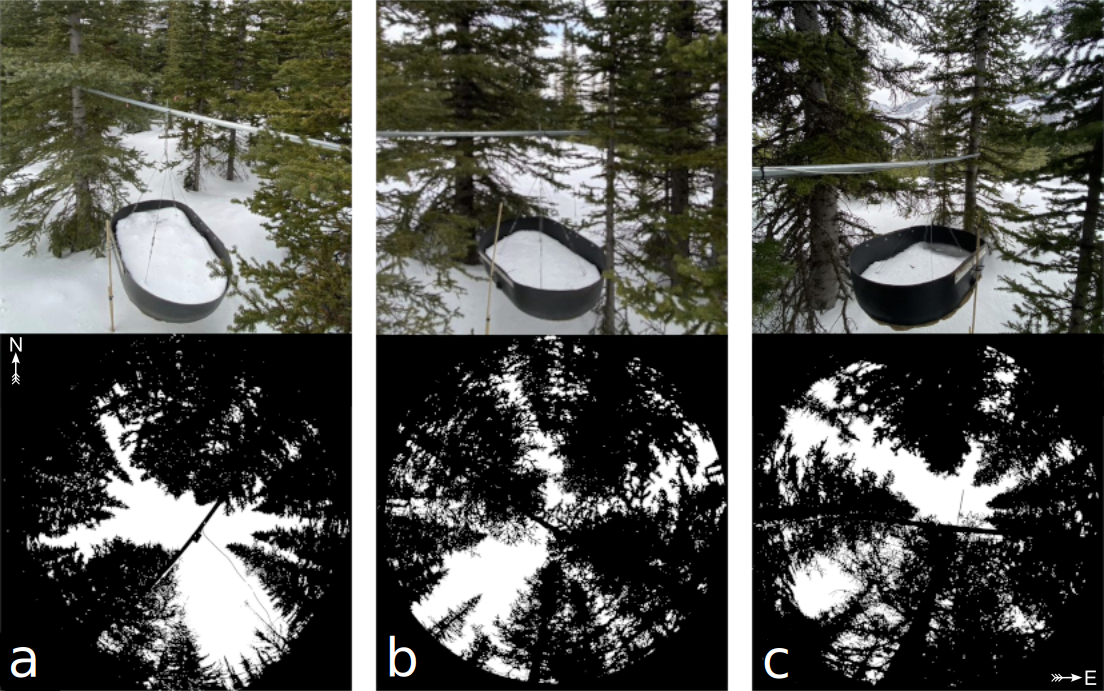
\includegraphics{figs/site-photos/scl_w_fisheye_textnew.png}

}

\caption{\label{fig-scl-imgs}Images of the three subcanopy lysimeters
(SCL) and surrounding canopy located in sparse (a), mixed (b), and dense
(c) canopy. The top row presents a side view of each SCL and the bottom
row shows hemispherical photographs classified using the hemispheR R
package. These hemispherical images are oriented with north at the top
and have been mirrored to provide a view from above (e.g., east is on
the right side of each image). See Table~\ref{tbl-scl-lai-cc} for the
canopy density measurements above each SCL.}

\end{figure}%

\subsection{UAV-Lidar data collection and
processing}\label{uav-lidar-data-collection-and-processing}

The UAV (FreeFly Alta X) payload included a REIGL miniVUX-2 airborne
laser scanner, an Applanix APX-20 inertial measurement unit (IMU) and
global navigation satellite system (GNSS). The UAV was flown 90 m above
the ground at a speed of 3 m s\textsuperscript{-1} following the path
shown in Figure~\ref{fig-site-map}. The methods outlined by Harder et
al. (2020) and Staines \& Pomeroy (2023) were incorporated to reconcile
survey lidar, IMU and GNSS data. A systematic vertical bias of up to 6
cm between UAV-lidar flight lines was observed in the resulting point
clouds on March 13\textsuperscript{th} and 14\textsuperscript{th}, 2024
and was attributed to IMU position drift. After strip alignment, the
mean elevation bias in the point clouds compared to the GNSS data was
0.000 m and the RMS error declined from 0.055 m to 0.038 m on March
13\textsuperscript{th} and changed from 0.033 m to 0.029 m on March
14\textsuperscript{th}. The point cloud density ranged from
\textasciitilde1200 returns m\textsuperscript{2} in sparse forest to
\textasciitilde2200 returns m\textsuperscript{2} in open clearings.
Quality control, ground classification, calculation of surface elevation
change was conducted on the point cloud data and then converted to 0.05
m resolution rasters. Further quality control was conducted on the 0.05
m raster data to remove values that exceeded the .999th quantile and
then resampled to 0.25 m grid cell resolution by taking the median. A
detailed description of the UAV, payload, flight settings, and software
packages used is provided in the supporting information.

\subsection{Snow surveys}\label{snow-surveys}

\subsubsection{In-situ snow depth and
density}\label{in-situ-snow-depth-and-density}

Event-based snow surveys provided measurements of subcanopy throughfall
depth and density at 30 locations following the transects shown in
Figure~\ref{fig-site-map}. These measurements were used to upscale the
weighed tree from kg to kg m\textsuperscript{-2}, assess the accuracy of
lidar derived snow depth measurements, and provide a fresh snow density
for the calculation of SWE (mm). Minimal ablation and redistribution of
both the surface snowpack and/or snow intercepted in the canopy was
crucial to ensure the snow survey measurements were attributed to
throughfall. Therefore, only snowfall events with minimal canopy snow
ablation as determined through in-situ observations, analysis of
timelapse imagery, and mass change on the weighed tree lysimeter were
selected. Twelve select in-situ fresh snow surveys (six pre- and
post-snowfall event pairs) conducted between January and May were used
to upscale the weighed tree from kg to kg m\textsuperscript{-2}. In-situ
snow surveys were also conducted following the UAV-lidar flights on
March 13\textsuperscript{th} and March 14\textsuperscript{th}. A 1000
cm\textsuperscript{3} Perla snow density wedge sampler (RIP Cutter,
https://snowmetrics.com/shop/rip-1-cutter-1000-cc/) was used to measure
the density of the fresh snow layer, \(\overline{\rho_{tf}}\) (kg
m\textsuperscript{-3}) from snow pits. Throughfall depth measurements,
\(\Delta HS\) were converted to SWE using the following equation:

\begin{equation}\phantomsection\label{eq-swe-tf}{
\Delta SWE_{tf} = \Delta HS \cdot \overline{\rho_{tf}}
}\end{equation}

If a pre-event crust layer was present, the depth of post event fresh
snow accumulation above the crust layer was interpreted as throughfall
over the event. In the absence of a defined crust layer, the difference
in pre- and post-event snow depth to ground was interpreted as event
throughfall.

\subsubsection{UAV-Lidar snow depth}\label{uav-lidar-snow-depth}

Two uncrewed aerial vehicle (UAV) lidar surveys were conducted before
and after a 24-hour snowfall event that occurred between March
13\textsuperscript{th} and March 14\textsuperscript{th}, 2023 to
facilitate the measurement of snow accumulation and canopy density
within the FT and PWL forest plots. This period was selected based on
two criteria: 1) it provided sufficient cumulative snowfall to result in
a low relative error in UAV-lidar measured throughfall, and 2) minimal
snow redistribution and ablation was observed, as confirmed by the SCLs,
weighed tree, and time-lapse imagery. The change in surface elevation
between the two UAV-lidar point clouds was interpreted as the increase
in snow accumulation, \(\Delta HS\) over the snowfall event.
\(\Delta SWE_{tf}\) was calculated using Equation~\ref{eq-swe-tf}
together with in-situ measurements of \(\overline{\rho_{tf}}\). The
measurement error of the UAV-lidar derived \(\Delta HS\) was assessed
using the in-situ snow depth observations which is shown in the
supporting information. Spatially distributed measurements of
\(\frac{I}{P}\), were then determined using Equation~\ref{eq-ip2} by
using \(\Delta SWE_{tf}\) as the throughfall component
(\(q_{tf} \Delta t\)) and the snowfall accumulation to the open
(\(q_{sf} \Delta t\)) measured between the two lidar surveys at PWL
station.

\subsection{UAV-Lidar canopy metrics}\label{uav-lidar-canopy-metrics}

The canopy of two UAV-lidar point clouds (March 13\textsuperscript{th}
and March 14\textsuperscript{th}) was characterized using the voxel ray
sampling (VoxRS) methodology for lidar data analysis, as developed by
Staines \& Pomeroy (2023). This method was chosen for its ability to
provide canopy metrics that are less sensitive to the inherent
non-uniform nature of lidar sampling data, which often results from beam
occlusion in vegetation and leads to reduced points near the ground.
Using this method radiation transmittance, \(\tau\) (-), was measured
across the hemisphere at a 1° step, e.g., azimuth angles (0°, 1°,
\ldots, 359°) and zenith angles (0°, 1°, \ldots, 90°) for each 0.25 m
grid cell within the FT and PWL forest plots. The fraction of snow-leaf
contact area per unit area of ground proposed by Hedstrom \& Pomeroy
(1998), and hereafter called leaf contact area (\(C_p\)), was then
calculated as:

\begin{equation}\phantomsection\label{eq-lca}{
C_p(C_c, \theta_h, L) = 1-\tau
}\end{equation}

\begin{equation}\phantomsection\label{eq-tf-ode}{
C_p(C_c, \theta_h, L) = \begin{cases}
    1-\tau,& \text{if } \theta_h> 0°\\
    1-\tau \approx C_c ,              & \theta_h= 0°
\end{cases}
}\end{equation}

where \(C_p\) is a function of the canopy cover \(C_c\), \(\theta_h\)
and \(L\). \(C_c\) is the fraction of canopy area to total ground area
when viewed from above, which differs from canopy closure, an
angular-derived metric usually measured from the ground perspective.

To determine how \(C_p\) was associated with interception efficiency at
different azimuth and zenith angles over the March 13--14 snowfall
event, the entire hemisphere at each grid location was considered. The
relationship between interception efficiency and \(C_p\) was found to be
linear and thus the Pearson Correlation Coefficient was used. The
\(\rho_p\) was computed between a single raster of interception
efficiency and each of the 32,760 rasters of \(C_p\) measured on March
13\textsuperscript{th}, representing locations across the hemisphere
(azimuth {[}0°, 1°, \ldots, 359°{]}, zenith angle {[}0°, 1°, \ldots,
90°{]}) at 0.25 m grid cells spanning the FT and PWL forest plots.

\subsection{Statistics and regression
models}\label{statistics-and-regression-models}

Linear and non-linear regression models were developed to assess
relationships in the observed data. Linear models were fitted using
ordinary least squares regression to analyze two relationships: (1)
between interception efficiency and meteorological variables and (2)
between interception efficiency and leaf contact area. The latter was
forced through the origin based on the theoretical justification that
the dependent variable should be zero when the independent variable is
zero. Kozak \& Kozak (1995) noted, the default
\emph{R}\textsuperscript{2} value provided for least squares models
forced through the origin by many statistical packages can be
misleading. Therefore, these \emph{R}\textsuperscript{2} values were
adjusted using Equation 10 in Kozak \& Kozak (1995). Non-linear models
were fitted to investigate the relationship of leaf contact area with
simulated trajectory angle using non-linear least squares regression.
All statistical analyses were conducted using the R `stats' package (R
Core Team, 2024).

\section{Results}\label{results}

\subsection{The influence of meteorology on snow
interception}\label{the-influence-of-meteorology-on-snow-interception}

Canopy snow load was estimated using the SCLs and weighed tree lysimeter
for 26 snowfall events and increased linearly with cumulative event
snowfall, showing no evidence of reaching a maximum
(Figure~\ref{fig-scl-w-sf}). Over these events, air temperature ranged
from -24.5°C to 1°C, wind speeds at 4.3 m height ranged from calm to 4.6
m s\textsuperscript{-1} (Table~\ref{tbl-sf-event-met}), and wind
direction was predominately from the southwest during snowfall
(Figure~\ref{fig-wind-rose}). Missing canopy snow load measurements in
Figure~\ref{fig-scl-w-sf} for certain events was caused by damage to the
wiring due to animals and heavy snow loads. Some of the the variability
in interception rates within and between different events may be
attributed to small amounts of canopy snow unloading and melt, which
could not be fully accounted for through the manual and automated
filtering mitigation strategies for in both the SCL and weighed tree
measurements. Additionally, the weighed tree lysimeter was influenced by
canopy snow sublimation, which was not directly accounted for in our
analysis.

\begin{figure}[H]

\centering{

\includegraphics{figs/automated_snowfall_event_periods/cuml_event_snowfall_canopy_storage_avg_of_scls_and_w_tree.png}

}

\caption{\label{fig-scl-w-sf}Plot showing the cumulative event snowfall
versus the corresponding state of canopy snow load calculated using the
average of the three subcanopy lysimeters (SCL, left) and weighed tree
lysimeter (right) for each of the 26 snowfall events.}

\end{figure}%

\pagebreak
\setstretch{1.0}

\begin{table}

\caption{\label{tbl-sf-event-met}Meteorology of the 26 snowfall events.
Air temperature and wind speed were measured at FT station. Interception
efficiency is estimated from snowfall measured at PWL station and the
average throughfall of all three SCLs located within the FT forest plot
(all from 15-min. measurements).}

\centering{

\fontsize{12.0pt}{14.4pt}\selectfont
\begin{tabular*}{\linewidth}{@{\extracolsep{\fill}}>{\centering\arraybackslash}p{\dimexpr 67.50pt -2\tabcolsep-1.5\arrayrulewidth}>{\centering\arraybackslash}p{\dimexpr 37.50pt -2\tabcolsep-1.5\arrayrulewidth}>{\centering\arraybackslash}p{\dimexpr 37.50pt -2\tabcolsep-1.5\arrayrulewidth}>{\centering\arraybackslash}p{\dimexpr 37.50pt -2\tabcolsep-1.5\arrayrulewidth}>{\centering\arraybackslash}p{\dimexpr 37.50pt -2\tabcolsep-1.5\arrayrulewidth}>{\centering\arraybackslash}p{\dimexpr 37.50pt -2\tabcolsep-1.5\arrayrulewidth}>{\centering\arraybackslash}p{\dimexpr 37.50pt -2\tabcolsep-1.5\arrayrulewidth}>{\centering\arraybackslash}p{\dimexpr 37.50pt -2\tabcolsep-1.5\arrayrulewidth}>{\centering\arraybackslash}p{\dimexpr 37.50pt -2\tabcolsep-1.5\arrayrulewidth}>{\centering\arraybackslash}p{\dimexpr 37.50pt -2\tabcolsep-1.5\arrayrulewidth}>{\centering\arraybackslash}p{\dimexpr 60.00pt -2\tabcolsep-1.5\arrayrulewidth}}
\toprule
 & \multicolumn{3}{>{\centering\arraybackslash}m{\dimexpr 112.50pt -2\tabcolsep-1.5\arrayrulewidth}}{Air Temperature (°C)} & \multicolumn{3}{>{\centering\arraybackslash}m{\dimexpr 112.50pt -2\tabcolsep-1.5\arrayrulewidth}}{Wind Speed (m/s)} & \multicolumn{3}{>{\centering\arraybackslash}m{\dimexpr 112.50pt -2\tabcolsep-1.5\arrayrulewidth}}{Interception Efficiency (-)} & Snowfall (mm) \\ 
\cmidrule(lr){2-4} \cmidrule(lr){5-7} \cmidrule(lr){8-10} \cmidrule(lr){11-11}
Start Date & Min & Mean & Max & Min & Mean & Max & Min & Mean & Max & Total \\ 
\midrule\addlinespace[2.5pt]
2021-12-23 & -6.2 & -5.3 & -4.6 & 0.6 & 3.1 & 4.6 & 0.1 & 0.5 & 0.9 & 21.7 \\ 
2022-01-02 & -15.9 & -10.8 & -5.8 & 0.2 & 1.8 & 4.2 & 0.0 & 0.5 & 1.0 & 31.6 \\ 
2022-01-17 & -14.8 & -7.4 & -0.7 & 0.2 & 1.1 & 1.8 & 0.0 & 0.5 & 0.9 & 12.0 \\ 
2022-01-31 & -24.5 & -12.1 & -6.4 & 0.1 & 1.0 & 1.7 & 0.2 & 0.7 & 1.0 & 9.1 \\ 
2022-02-14 & -9.9 & -9.0 & -8.5 & 0.4 & 0.8 & 1.2 & 0.2 & 0.5 & 0.8 & 1.7 \\ 
2022-02-19 & -4.7 & -3.2 & -2.5 & 1.3 & 2.3 & 3.6 & 0.3 & 0.6 & 0.9 & 11.1 \\ 
2022-03-01 & -8.3 & -5.4 & -1.0 & 0.1 & 1.0 & 3.1 & 0.1 & 0.6 & 1.0 & 9.8 \\ 
2022-03-07 & -12.5 & -8.5 & -3.5 & 0.3 & 0.8 & 1.7 & 0.0 & 0.6 & 1.0 & 9.5 \\ 
2022-03-14 & -2.7 & -2.1 & -0.8 & 1.0 & 1.6 & 2.9 & 0.2 & 0.6 & 0.9 & 8.4 \\ 
2022-03-19 & -3.1 & -2.8 & -2.5 & 0.0 & 0.7 & 1.3 & 0.3 & 0.5 & 0.6 & 6.6 \\ 
2022-03-23 & -7.9 & -5.3 & -0.9 & 0.8 & 1.2 & 1.8 & 0.4 & 0.6 & 0.9 & 1.6 \\ 
2022-04-04 & -3.5 & -2.9 & -2.1 & 0.6 & 1.0 & 1.9 & 0.0 & 0.4 & 0.6 & 3.4 \\ 
2022-04-18 & -5.2 & -4.0 & -2.7 & 0.4 & 1.1 & 1.9 & 0.1 & 0.5 & 0.9 & 7.4 \\ 
2022-04-22 & -2.8 & -1.8 & -0.5 & 0.4 & 0.8 & 1.2 & 0.1 & 0.5 & 1.0 & 9.8 \\ 
2022-05-09 & -4.9 & -4.3 & -3.2 & 0.1 & 0.4 & 0.9 & 0.2 & 0.5 & 0.9 & 8.1 \\ 
2022-05-19 & -4.9 & -2.1 & 0.3 & 0.1 & 0.4 & 0.9 & 0.2 & 0.6 & 0.9 & 7.1 \\ 
2022-06-13 & -1.1 & -0.3 & 0.6 & 0.1 & 0.1 & 0.4 & 0.0 & 0.5 & 0.9 & 45.4 \\ 
2022-12-27 & -3.0 & -2.7 & -1.9 & 0.6 & 1.1 & 1.8 & 0.2 & 0.5 & 0.9 & 4.5 \\ 
2023-01-27 & -11.5 & -7.3 & -4.5 & 0.6 & 0.9 & 1.2 & 0.1 & 0.5 & 0.8 & 10.4 \\ 
2023-02-19 & -14.3 & -9.4 & -6.3 & 0.2 & 0.8 & 1.4 & 0.3 & 0.6 & 1.0 & 17.7 \\ 
2023-02-26 & -9.2 & -8.4 & -6.6 & 0.2 & 1.0 & 2.1 & 0.3 & 0.5 & 1.0 & 5.4 \\ 
2023-03-13 & -8.9 & -3.6 & -0.1 & 0.3 & 1.3 & 2.2 & 0.0 & 0.5 & 1.0 & 27.4 \\ 
2023-03-24 & -7.9 & -5.7 & -3.5 & 0.1 & 0.5 & 1.2 & 0.1 & 0.4 & 0.7 & 23.8 \\ 
2023-04-01 & -8.9 & -7.7 & -4.7 & 0.1 & 0.6 & 1.4 & 0.4 & 0.6 & 0.8 & 11.4 \\ 
2023-04-10 & -1.1 & -0.5 & 0.3 & 0.1 & 0.3 & 1.0 & 0.4 & 0.6 & 0.8 & 18.0 \\ 
2023-05-08 & 0.2 & 0.6 & 1.0 & 0.4 & 0.6 & 0.8 & 0.5 & 0.5 & 0.7 & 3.5 \\ 
\bottomrule
\end{tabular*}

}

\end{table}%

\setstretch{1.5}

\begin{figure}[H]

\centering{

\includegraphics[width=0.6\textwidth,height=\textheight]{figs/automated_snowfall_event_periods/ft_wind_rose_allevents_snowing_custom_dimensions.png}

}

\caption{\label{fig-wind-rose}Wind rose showing the frequency of wind
speed and direction over the 26 snowfall periods for the ultrasonic
anemometer 4.3 m above ground at FT station.}

\end{figure}%

Event average air temperature and interception efficiency were
negatively associated for the mixed canopy (\emph{R}\textsuperscript{2}
= 0.1, \emph{p} \textless{} 0.05), but not associated at the closed and
sparse canopies (Table~\ref{tbl-lysimeter-event-stats} \&
Figure~\ref{fig-scl-ip-avg-event}). Cumulative event snowfall was not
associated with event interception efficiency at any site (\emph{p}
\textgreater{} 0.05). Event wind speed was positively associated with
interception efficiency for the sparse (\emph{R}\textsuperscript{2} =
0.1, \emph{p} \textgreater{} 0.05) and closed
(\emph{R}\textsuperscript{2} = 0.2, \emph{p} \textless{} 0.05) canopies,
both with limited canopy openings (Figure 2a,c) towards the prevailing
wind direction shown in the wind rose in Figure~\ref{fig-wind-rose}.
However, interception efficiency in the mixed canopy, which is partially
open towards the prevailing wind direction, was not associated with wind
speed (\emph{p} \textgreater{} 0.05).

\begin{figure}[H]

\centering{

\includegraphics{figs/automated_snowfall_event_periods/event_avg_temp_wind_cuml_snow_vs_IP_colour_troughs.png}

}

\caption{\label{fig-scl-ip-avg-event}Scatter plots showing the event
mean air temperature, mean wind speed, and cumulative snowfall versus
the event mean interception efficiency estimated using the SCLs for each
of the 26 snowfall events. The colours (grey, yellow, and green),
correspond to varying canopy closure (0.64, 0.75, and 0.79). A linear
regression line fit to the data for significant relationships (\emph{p}
\textless{} 0.05) is shown by the solid coloured lines. See
Table~\ref{tbl-lysimeter-event-stats} for linear regression statistics.}

\end{figure}%

\begin{longtable}[]{@{}
  >{\raggedright\arraybackslash}p{(\columnwidth - 10\tabcolsep) * \real{0.3623}}
  >{\raggedright\arraybackslash}p{(\columnwidth - 10\tabcolsep) * \real{0.1304}}
  >{\raggedright\arraybackslash}p{(\columnwidth - 10\tabcolsep) * \real{0.0870}}
  >{\raggedleft\arraybackslash}p{(\columnwidth - 10\tabcolsep) * \real{0.2174}}
  >{\raggedleft\arraybackslash}p{(\columnwidth - 10\tabcolsep) * \real{0.1449}}
  >{\raggedleft\arraybackslash}p{(\columnwidth - 10\tabcolsep) * \real{0.0580}}@{}}

\caption{\label{tbl-lysimeter-event-stats}Statistics corresponding to
the ordinary least squares linear regression test between independent
variables: mean event air temperature, cumulative event snowfall, and
mean event wind speed, and the dependent variable mean event
interception efficiency. The test was run separately for three levels of
canopy closure (\(C_c\)) and for the average of all three SCLs
(scl\_mean).}

\tabularnewline

\toprule\noalign{}
\begin{minipage}[b]{\linewidth}\raggedright
Dependent Variable
\end{minipage} & \begin{minipage}[b]{\linewidth}\raggedright
SCL Name
\end{minipage} & \begin{minipage}[b]{\linewidth}\raggedright
\(C_c\)
\end{minipage} & \begin{minipage}[b]{\linewidth}\raggedleft
Adjusted \(R^2\)
\end{minipage} & \begin{minipage}[b]{\linewidth}\raggedleft
\(p\)-value
\end{minipage} & \begin{minipage}[b]{\linewidth}\raggedleft
\(n\)
\end{minipage} \\
\midrule\noalign{}
\endhead
\bottomrule\noalign{}
\endlastfoot
Air Temperature (°C) & closed & 0.79 & 0.008 & 0.296 & 20 \\
Air Temperature (°C) & mixed & 0.75 & 0.141 & 0.033 & 26 \\
Air Temperature (°C) & sparse & 0.64 & -0.033 & 0.520 & 19 \\
Air Temperature (°C) & scl\_mean & 0.73 & 0.039 & 0.168 & 26 \\
Cumulative Snowfall (mm) & closed & 0.79 & -0.049 & 0.733 & 20 \\
Cumulative Snowfall (mm) & mixed & 0.75 & 0.029 & 0.198 & 26 \\
Cumulative Snowfall (mm) & sparse & 0.64 & -0.038 & 0.569 & 19 \\
Cumulative Snowfall (mm) & scl\_mean & 0.73 & 0.010 & 0.276 & 26 \\
Wind Speed (m/s) & closed & 0.79 & 0.192 & 0.031 & 20 \\
Wind Speed (m/s) & mixed & 0.75 & 0.010 & 0.274 & 26 \\
Wind Speed (m/s) & sparse & 0.64 & 0.114 & 0.087 & 19 \\
Wind Speed (m/s) & scl\_mean & 0.73 & -0.020 & 0.479 & 26 \\

\end{longtable}

Fifteen-minute interval measurements of interception efficiency and air
temperature shown in Figure 6a were not associated, despite significant
relationships for the sparse and mixed canopies
(\emph{R}\textsuperscript{2} \textless{} 0.03, \emph{p} \textless{}
0.05), due to low predictive power
(Table~\ref{tbl-lysimeter-15min-stats}). The average interception
efficiency across differing bins of air temperature also does not show
any systematic trend (Figure 6a). However, a significantly greater
median interception efficiency (\emph{p} \textless{} 0.05) was found for
binned measurements with air temperatures below -6 °C compared to those
with warmer air temperatures using non-parametric Wilcoxon signed rank
test.

Mean wind speed was weakly associated with interception efficiency for
the sparse (\emph{R}\textsuperscript{2} = 0.1, \emph{p} \textgreater{}
0.05) and closed (\emph{R}\textsuperscript{2} = 0.2, p \textless{}
0.05), but not for the mixed canopy (\emph{p} \textgreater{} 0.05)
(Table~\ref{tbl-lysimeter-15min-stats}). The binned data show an
increasing trend in interception efficiency with increasing wind speed
for the sparse and closed canopies (Figure 6b). A comparison of
interception efficiencies binned for low (\textless{} 1 m
s\textsuperscript{-1}) and high (\textgreater{} 1 m
s\textsuperscript{-1}) wind speeds by the Wilcoxon signed rank test,
showed that high wind speeds had significantly higher (\emph{p}
\textless{} 0.05) median interception efficiencies compared to the low
wind speed bins for the closed and sparse canopy. Conversely, the
Wilcoxon test showed the mixed canopy, which had an opening in the
canopy towards the prevailing wind direction (Figure 2b), had
significantly higher (\emph{p} \textless{} 0.05) median interception
efficiencies for the low wind speed bins.

Interception efficiency showed no association
(\emph{R}\textsuperscript{2} \textless{} 0.05, \emph{p} \textgreater{}
0.2) with the canopy load measured at the beginning of the 15-minute
intervals (Table~\ref{tbl-lysimeter-15min-stats}). The binned data show
a small increase in interception efficiency for all three canopies when
the snow load is less than 7 mm (Figure 6c). Interception efficiency
later declined for snow loads greater than 7 mm for all canopies, though
this was inconsistent for the mixed canopy. A significantly greater
(\emph{p} \textless{} 0.05) median interception efficiency was found for
canopy snow loads less than 10 mm than those with high initial canopy
snow loads (\textgreater{} 10 mm) using the Wilcoxon rank-test.
Additional statistics from ordinary least squares regression test on the
15-minute interval measurements are provided in
Table~\ref{tbl-lysimeter-15min-stats}.

\begin{figure}[H]

\centering{

\includegraphics{figs/automated_snowfall_event_periods/troughs_met_vs_IP_bin.png}

}

\caption{\label{fig-scl-ip-avg-15min}Scatter plots of 15-minute interval
measurements (blue dots) and binned data (black open circles with error
bars) of mean air temperature, mean wind speed, and initial canopy snow
load versus mean snow interception efficiency. Panels show (a) air
temperature, (b) wind speed, and (c) initial canopy snow load (the snow
load observed at the beginning of the timestep). The black open circles
show the mean of each bin and the error bars represent the standard
deviations. See Table~\ref{tbl-lysimeter-15min-stats} for linear
regression statistics.}

\end{figure}%

\begin{longtable}[]{@{}
  >{\raggedright\arraybackslash}p{(\columnwidth - 10\tabcolsep) * \real{0.4000}}
  >{\raggedright\arraybackslash}p{(\columnwidth - 10\tabcolsep) * \real{0.1200}}
  >{\raggedleft\arraybackslash}p{(\columnwidth - 10\tabcolsep) * \real{0.0800}}
  >{\raggedleft\arraybackslash}p{(\columnwidth - 10\tabcolsep) * \real{0.2000}}
  >{\raggedleft\arraybackslash}p{(\columnwidth - 10\tabcolsep) * \real{0.1333}}
  >{\raggedleft\arraybackslash}p{(\columnwidth - 10\tabcolsep) * \real{0.0667}}@{}}

\caption{\label{tbl-lysimeter-15min-stats}Statistics corresponding to
the ordinary least squares linear regression test between 15-minute
interval measurements of independent variables: mean air temperature,
mean wind speed, and initial canopy snow load and the dependent variable
mean interception efficiency. The test was run separately for three
levels of canopy closure (\(C_l\)).}

\tabularnewline

\toprule\noalign{}
\begin{minipage}[b]{\linewidth}\raggedright
Dependent Variable
\end{minipage} & \begin{minipage}[b]{\linewidth}\raggedright
SCL Name
\end{minipage} & \begin{minipage}[b]{\linewidth}\raggedleft
\(C_l\)
\end{minipage} & \begin{minipage}[b]{\linewidth}\raggedleft
Adjusted \(R^2\)
\end{minipage} & \begin{minipage}[b]{\linewidth}\raggedleft
\(p\)-value
\end{minipage} & \begin{minipage}[b]{\linewidth}\raggedleft
\(n\)
\end{minipage} \\
\midrule\noalign{}
\endhead
\bottomrule\noalign{}
\endlastfoot
Air Temperature (°C) & Mixed & 0.75 & 0.026 & 0.000 & 1001 \\
Air Temperature (°C) & Closed & 0.79 & 0.011 & 0.002 & 830 \\
Air Temperature (°C) & Sparse & 0.64 & 0.011 & 0.006 & 609 \\
Wind Speed (m/s) & Mixed & 0.75 & 0.016 & 0.000 & 1001 \\
Wind Speed (m/s) & Closed & 0.79 & 0.026 & 0.000 & 830 \\
Wind Speed (m/s) & Sparse & 0.64 & 0.085 & 0.000 & 609 \\
Initial Canopy Snow Load (mm) & Mixed & 0.75 & 0.007 & 0.006 & 987 \\
Initial Canopy Snow Load (mm) & Closed & 0.79 & 0.012 & 0.001 & 815 \\
Initial Canopy Snow Load (mm) & Sparse & 0.64 & 0.038 & 0.000 & 598 \\

\end{longtable}

\subsection{The influence of forest structure on snow
interception}\label{the-influence-of-forest-structure-on-snow-interception}

UAV-lidar measurements of throughfall and canopy density provide
insights on how the forest canopy influenced subcanopy snow accumulation
during a wind-driven snowfall event between March 13\textsuperscript{th}
and 14\textsuperscript{th} 2023. This event totaled 28.7 mm of snowfall
at PWL station and was characterized by a transition from low rates of
snowfall and air temperatures near 0°C to higher rates of snowfall by
late afternoon on March 13\textsuperscript{th} coinciding with air
temperatures around -2.5 °C. An average wind speed of 1.3 m
s\textsuperscript{-1} and direction of 188° was observed 4.3 m above the
ground at FT Station. Figure~\ref{fig-wind-profiles} shows the wind
speed profile fit to the Prandtl-von Kármán log-linear relationship
which differs from other wind speed profiles developed in dense canopy
(e.g, Cionco, 1965). The predicted hydrometeor trajectory angles at
varying heights, calculated using Equation~\ref{eq-ta} and the mean
observed hydrometeor terminal velocity observed over the event of 0.9 m
s\textsuperscript{-1} are also shown in Figure~\ref{fig-wind-profiles}.
An average wind speed of 1.6 m s\textsuperscript{-1} and direction of
188° was calculated by integrating the wind speed from the surface to
the mean canopy height of FT plot. The corresponding trajectory angle
calculated using Equation~\ref{eq-ta} from this integrated wind speed
was 61.5°.

\begin{figure}[H]

\centering{

\includegraphics{figs/lidar_periods/wind_profile_w_trajectories_20230313.png}

}

\caption{\label{fig-wind-profiles}Wind speed profile using roughness
length and displacement height parameters derived from anemometers at 2,
3, 4.3, and 13.5 m above ground at FT station over snow free periods and
friction velocity estimated over the March 13--14\textsuperscript{th}
snowfall event.}

\end{figure}%

Throughfall depth measured by UAV-lidar was close to the 28 in-situ
manual measurements with a mean bias of -0.001 m and RMSE of 0.024 m.
More details on the accuracy of UAV-lidar snowdepth measurements are
provided in the supporting information section.
Figure~\ref{fig-lidar-tf-ip} shows the spatial distribution of
throughfall and interception efficiency at the PWL and FT forest plots.
Reduced throughfall and greater interception efficiency was observed on
the north (lee) side of individual trees, which may be due to
non-vertical hydrometeor trajectories caused by the steady southerly
winds observed over this event. Transparent areas within the forest
plots in Figure~\ref{fig-lidar-tf-ip} represent grid cells that did not
have any lidar ground returns (e.g., under dense canopy proximal to tree
trunks) or were masked due to disturbance (e.g., walking paths in
clearings). Visual observations on March 13\textsuperscript{th} and
14\textsuperscript{th} confirmed non-vertical hydrometeor trajectories
and increased canopy snow loads were observed on the windward side of
individual trees. This effect is shown in Figure~\ref{fig-lidar-tf-ip}
to be more apparent in the PWL forest plot than the FT forest plot. This
may be attributed to the taller trees and higher canopy cover of the PWL
forest plot compared to the FT forest plot, as for the same trajectory
angle a taller tree will produce a larger downwind footprint.

\begin{figure}[H]

\centering{

\includegraphics{figs/external_figures/facet_ft_pwl_23_072_23_073_v2.0.0_saswe_and_ip_normalised_resample_0.25.png}

}

\caption{\label{fig-lidar-tf-ip}UAV-lidar measurements of the change in
snow water equivalent, SWE (mm) and interception efficiency, I/P (-),
over the March 13, 2023 24-hour snowfall event for the FT and PWL forest
plots at a 0.25 m resolution. See the location of the two forest plots
in Figure~\ref{fig-site-map}.}

\end{figure}%

Figure~\ref{fig-hemi-ip-cc} shows a strong linear correlation between
\(C_p\) and interception efficiency towards the southern portion of the
hemisphere, aligning with the average event wind direction. For the PWL
forest plot, the upper 97.5\textsuperscript{th} percentile of the
\(\rho_p\) values shown in Figure~\ref{fig-hemi-ip-cc}, were found
between azimuth angles of 167°--217°. Similarly, for the FT forest plot,
the upper 97.5\textsuperscript{th} percentile of \(\rho_p\) was found
between azimuth angles of 171°--223°. The zenith angle found to have the
highest correlation over this azimuth range was 22° (\(\rho_p\) = 0.7)
and 21° (\(\rho_p\) = 0.83) for PWL and FT respectively. The high
correlation coefficients found for non-vertical zenith angles for both
PWL and FT are hypothesized to result from non-vertical hydrometeor
trajectories.

\begin{figure}[H]

\centering{

\includegraphics{figs/external_figures/full_hemi_rho_p_cor_lca_ip_23_072_vox_len_0.25m_sa_gridgen_v2.0.0_sa_ft_pwl_.png}

}

\caption{\label{fig-hemi-ip-cc}The Pearson Correlation Coefficient
between rasters (0.25 m resolution) of interception efficiency and leaf
contact area for each grid cell across the study site for each azimuth
angles (0°, 1°, \ldots, 359°) and zenith angles (0°, 1°, \ldots, 90°)
for the FT (left) and PWL (right) forest plots.}

\end{figure}%

The correlation between \(C_p\) and interception efficiency, resampled
to a 5 m grid resolution, was higher when \(C_p\) was adjusted for the
observed shift in hydrometeor trajectory (Vector Based), compared to the
leaf contact angle measured at a zenith angle of 0° (nadir)
(Figure~\ref{fig-lca-vs-ip}). The azimuth and zenith angles observed to
have the highest \(\rho_p\) in Figure~\ref{fig-hemi-ip-cc} was used to
adjust the vector based, \(C_p\) in Figure~\ref{fig-lca-vs-ip}. The
stronger association for the vector-based calculation suggests that
adjusted \(C_p\) is a useful predictor of interception efficiency before
ablation. An ordinary least squares linear regression forced through the
origin was fit to the observed data points using the following equation:

\begin{equation}\phantomsection\label{eq-lca-ip}{
  \frac{I}{P} = C_p(C_c, \theta_h) \cdot \alpha
}\end{equation}

where \(\alpha\) is an efficiency constant which determines the fraction
of snowflakes that contact the \(C_p\) elements and are stored in the
canopy (e.g., intercepted) before canopy snow unloading or ablation
processes begin.

\begin{figure}[H]

\centering{

\includegraphics{figs/external_figures/pwl_ft_lca_vs_ip_phi_nadir_adjusted_resample_w_mods_5m.png}

}

\caption{\label{fig-lca-vs-ip}Scatter plots showing the relationship
between leaf contact area and interception efficiency rasters resampled
to a 5 m grid cell resolution. The left plot (nadir) shows leaf contact
area measured from a zenith angle of 0°. The right plot (Vector Based)
shows the leaf contact area averaged over rasters with zenith angles
(PWL = 22°, FT = 21°) and azimuth angles (PWL = 167°, 178°, \ldots{}
217°; FT = 171°, 172°, \ldots{} 223°). The solid lines (Model fit) show
an ordinary least squares linear regression forced through the origin
and fitted to the PWL (red) and FT (black) data and the light grey
dotted line shows a 1:1 line. The \emph{R}\textsuperscript{2} values for
the four different models are shown in the upper right of each panel
calculated following the methods outlined in Kozak \& Kozak (1995).}

\end{figure}%

For the vector-based model, the relationship between interception
efficiency and \(C_p\) results in \emph{R}\textsuperscript{2} values of
0.47 and 0.8 for PWL and FT respectively. The increase in interception
efficiency with \(C_p\) follows a reduced slope compared to the nadir
models with \(\alpha\) values of 0.71 and 0.68 for the PWL and FT
vector-based models respectively. The reduced slope for the vector-based
models may be due to snowflakes that weaved through and/or bounced off
branch elements in addition to UAV-lidar measurement uncertainty which
may have been slightly affected by unloading and redistribution. These
processes would have reduced the fraction of snowfall that was stored in
the canopy. Model error statistics are presented in
Table~\ref{tbl-ip-mod-err} for the nadir and vector-based models and
show the vector-based model provided a better prediction of interception
efficiency. Some of the scatter observed in the nadir model shown in
Figure~\ref{fig-lca-vs-ip} may be explained by grid cells which observed
a greater interception efficiency compared to the corresponding \(C_c\)
value and can be attributed to the inability of \(C_c\) to represent the
increase in interception observed within canopy gaps in
Figure~\ref{fig-lidar-tf-ip}. Conversely, grid cells where interception
efficiency is less than \(C_c\), may be affected by non-vertical
trajectory hydrometeors making their way underneath the canopy as
observed by the reduced interception efficiency on the windward edges of
individual trees in Figure~\ref{fig-lidar-tf-ip}. The latter explanation
suggests the non-linear relationship observed for the PWL nadir
calculation in Figure~\ref{fig-lidar-tf-ip}.

\pagebreak

\begin{longtable}[]{@{}
  >{\raggedright\arraybackslash}p{(\columnwidth - 12\tabcolsep) * \real{0.1149}}
  >{\raggedright\arraybackslash}p{(\columnwidth - 12\tabcolsep) * \real{0.2184}}
  >{\raggedleft\arraybackslash}p{(\columnwidth - 12\tabcolsep) * \real{0.1839}}
  >{\raggedleft\arraybackslash}p{(\columnwidth - 12\tabcolsep) * \real{0.1609}}
  >{\raggedleft\arraybackslash}p{(\columnwidth - 12\tabcolsep) * \real{0.0920}}
  >{\raggedleft\arraybackslash}p{(\columnwidth - 12\tabcolsep) * \real{0.1609}}
  >{\raggedleft\arraybackslash}p{(\columnwidth - 12\tabcolsep) * \real{0.0690}}@{}}

\caption{\label{tbl-ip-mod-err}Model error statistics provided for
predictions of interception efficiency using Equation~\ref{eq-lca-ip}
and for different \(a\) values, as shown in the Model Slope column.
Statistics are provided for the PWL and FT forest plots, using leaf
contact area canopy metrics adjusted to zenith angles of (0°, 1°,
\ldots{} 30°) and azimuth angles (170°, 171°, \ldots{} 220°) and nadir
zenith angle of 0°. The Mean bias is the difference in the model and
observed values, MAE is the mean of the absolute error, RMS Error is the
root mean squared error, \emph{R}\textsuperscript{2} is the coefficient
of determination adjusted using Equation 10 in Kozak \& Kozak (1995).}

\tabularnewline

\toprule\noalign{}
\begin{minipage}[b]{\linewidth}\raggedright
Plot Name
\end{minipage} & \begin{minipage}[b]{\linewidth}\raggedright
Canopy Calculation
\end{minipage} & \begin{minipage}[b]{\linewidth}\raggedleft
Model Slope (-)
\end{minipage} & \begin{minipage}[b]{\linewidth}\raggedleft
Mean Bias (-)
\end{minipage} & \begin{minipage}[b]{\linewidth}\raggedleft
MAE (-)
\end{minipage} & \begin{minipage}[b]{\linewidth}\raggedleft
RMS Error (-)
\end{minipage} & \begin{minipage}[b]{\linewidth}\raggedleft
\(R^2\)
\end{minipage} \\
\midrule\noalign{}
\endhead
\bottomrule\noalign{}
\endlastfoot
FT & Nadir & 0.99 & 0.022 & 0.071 & 0.099 & 0.51 \\
FT & Vector Based & 0.68 & 0.001 & 0.047 & 0.062 & 0.80 \\
PWL & Nadir & 0.95 & 0.048 & 0.113 & 0.146 & NA \\
PWL & Vector Based & 0.71 & 0.019 & 0.078 & 0.095 & 0.47 \\

\end{longtable}

\subsection{The combined influence of trajectory angle and forest
structure on
interception}\label{the-combined-influence-of-trajectory-angle-and-forest-structure-on-interception}

Figure~\ref{fig-lca-ht-ws} shows that \(C_p\), measured from VoxRS prior
to snowfall on March 13\textsuperscript{th}, increases substantially
with simulated hydrometeor trajectory angle and corresponding simulated
wind speed. The standard deviation in VoxRS measured \(C_p\),
illustrated by the shaded area in Figure~\ref{fig-lca-ht-ws}, exhibits
the broad range in values for individual grid cells across each forest
plot. Despite this large scatter, a systematic increase in the mean
\(C_p\) across both forest plots results from a rise in the number of
canopy elements for more horizontal angles, when averaged across each
forest plot, over all azimuth angles (see top left panel
Figure~\ref{fig-lca-ht-ws}). This results in a large rise in \(C_p\)
over relatively common estimated wind speeds. For example, with a wind
speed of 1 m s\textsuperscript{-1} and estimated trajectory angle of
48°, \(C_p\) would increase by 0.31 and 0.28 for the PWL and FT forest
plots respectively (Figure~\ref{fig-lca-ht-ws}). This is a fractional
increase in the plot \(C_p\) from nadir of 0.61 and 0.95 for PWL and FT
respectively. The increase in \(C_p\) from \(C_c\), with increasing
trajectory angle is shown on the bottom row of
Figure~\ref{fig-lca-ht-ws} and exhibits a similar relationship for both
forest plots FT and PWL until trajectory angles reach approximately 60°.
Beyond 60°, the PWL rate of increase slows as the \(C_p\) approaches
1.0, while the FT plot, which has lower \(C_c\), continues to rise until
around 75° as a \(C_p\) of 1.0 is approached. \(C_p\) was also
quantified across trajectory angles for both PWL and FT on March
14\textsuperscript{th}, post snowfall, and showed a negligible increase
in \(C_p\) compared to \(C_p\) measured on March 13\textsuperscript{th}
without snow in the canopy.

\begin{figure}[H]

\centering{

\includegraphics{figs/external_figures/WITH_TREEWELLS_traj_angle_and_wind_single_zenith_1_thetaby_1_traj_angle_wind_speed_vs_cowplot_lca_and_inc_w_mods_mean_sd_23_072.png}

}

\caption{\label{fig-lca-ht-ws}Plots showing the relationship between
hydrometeor trajectory angle (left column) and wind speed (right column)
with mean plot-wide snow-leaf contact area, \(C_p\) (top row) and the
increase in mean plot-wide \(C_p\), e.g., \(C_p - C_c\) (bottom row).
The simulated hydrometeor trajectory angle is measured as degrees from
zenith. Simulated wind speed was calculated as a function of hydrometeor
trajectory angle by rearranging Equation~\ref{eq-ta} and an observed
event hydrometeor fall velocity of 0.9 m s\textsuperscript{-1}. The
solid lines (VoxRS) represent the mean \(C_p\) (top row) or increase in
mean \(C_p\) (bottom row) for a single zenith angle observed from VoxRS
across all grid cells for each forest plot and across all azimuth
angles. The shaded area represents 1 standard deviation above and below
the observed VoxRS mean. The dashed lines (Fitted) represent predictions
from Equation~\ref{eq-lca-ac} (top row) and Equation~\ref{eq-lca-inc}
(bottom row). The dotted lines (HP98) represent the predictions from
Equation 10 in Hedstrom \& Pomeroy (1998). A forested downwind distance
of 100 m was assumed for the HP98 calculation.}

\end{figure}%

A function is proposed here to calculate plot-scale leaf contact area,
\(C_p\) (-):

\begin{equation}\phantomsection\label{eq-lca-ac}{
C_p = C_c + C_{inc}(\theta_h, C_c)
}\end{equation}

where, \(C_{inc}\) represents the increase in leaf contact area from
\(C_c\), and it is a function of \(\theta_h\). To estimate \(C_{inc}\)
in the absence of detailed canopy measurements, the following function
is proposed:

\begin{equation}\phantomsection\label{eq-lca-inc}{
C_{inc} = (1-C_c)\cdot f(\theta_h)
}\end{equation}

where \(1-C_C\) represents the void space in the canopy, and
\(f(\theta_h)\) is a function describes the relative increase in canopy
area as a function of \(\theta_h\). Here, \(f(\theta_h)\) is
approximated here as:

\begin{equation}\phantomsection\label{eq-f-theta}{
f(\theta_h) = b \cdot\text{sin}(\theta_h)^2
}\end{equation}

where \(b\) is a fitting coefficient, estimated to be
\textasciitilde0.91 through a non-linear least squares regression fit to
the VoxRS measurements at both FT and PWL. The use of
\(\text{sin}(\theta_h)^2\) in Equation~\ref{eq-f-theta} reflects the
relative increase in snow-leaf contact area, which also leads to a
proportional decrease in the canopy void space (\(1-C_c\)). The
assumptions of Equation~\ref{eq-f-theta} include its application to a
forest with relatively uniform structure (e.g., without large clear
cuts) and where the mean height of the canopy is greater than the mean
width of individual trees.

Simulated \(C_p\) using Equation~\ref{eq-lca-ac} is shown in the dashed
lines in the top row of Figure~\ref{fig-lca-ht-ws} and follows the
VoxRS-measured mean \(C_p\) closely. Model error statistics shown in
Table~\ref{tbl-lca-mod-err} demonstrate that Equation~\ref{eq-lca-inc}
performed well, with a mean bias and RMSE of (-) and (-) respectively
for PWL, and (-) and (-) for FT. In contrast,
Table~\ref{tbl-lca-mod-err} reveals that the Hedstrom \& Pomeroy (1998)
method produced significantly less accurate estimates of \(C_p\), with a
mean bias and RMSE of -0.2 (-) and 0.23 (-) respectively for PWL, and
-0.26 (-) and 0.32 (-) for FT.

\begin{longtable}[]{@{}llrrrr@{}}

\caption{\label{tbl-lca-mod-err}Model error statistics calculated for
the prediction of leaf contact area from trajectory angle using
Equation~\ref{eq-lca-inc} (Eq. 11) and Equation 10 from Hedstrom \&
Pomeroy (1998) for the PWL and FT forest plots. Mean bias is the
difference in the model and observed values, MAE is the mean of the
absolute error, RMS Error is the root mean squared error and
\emph{R}\textsuperscript{2} is the coefficient of determination. The
units for all metrics are dimensionless. A forested downwind distance of
100 m was used for the HP98 calculation.}

\tabularnewline

\toprule\noalign{}
Model & Plot Name & Mean Bias (-) & MAE (-) & RMS Error (-) & \(R^2\) \\
\midrule\noalign{}
\endhead
\bottomrule\noalign{}
\endlastfoot
HP98 & FT & -0.26 & 0.26 & 0.32 & -0.97 \\
HP98 & PWL & -0.20 & 0.20 & 0.23 & -0.96 \\
Eq. 10 & FT & 0.03 & 0.04 & 0.05 & 0.95 \\
Eq. 10 & PWL & -0.05 & 0.05 & 0.05 & 0.90 \\

\end{longtable}

\subsection{Throughfall model
performance}\label{throughfall-model-performance}

The performance of Equations 9, 10, and 11 in estimating event
throughfall was assessed against UAV-lidar measurements of throughfall
for the March 13--14\textsuperscript{th} snowfall event at the plot
scale for both FT and PWL. Required values for the model included the
event mean hydrometeor terminal velocity and event total snowfall which
were measured at PWL station, and wind speed was taken as one-third the
mean canopy height using the wind speed profile in
Figure~\ref{fig-wind-profiles}. Additional model inputs include the mean
\(C_c\) for each plot which was measured from the VoxRS dataset. An
\(\alpha\) value of 0.874 (-) was found through calibration which
provided the best fit between observed and simulated interception
efficiency at the plot scale for both FT and PWL.

Figure~\ref{fig-event-tf} shows the vector-based model, computed using
Equation~\ref{eq-lca-ip} with \(C_p\) adjusted for estimated hydrometeor
trajectory angle, closely matches UAV-lidar measurements of throughfall.
Observed and modelled values of interception efficiency and
\(\Delta SWE_{tf}\) are presented in Table~\ref{tbl-vb-plot-err} along
with corresponding error statistics. Modelled throughfall from the
vector-based model was 17.5 mm compared to the measured throughfall of
16.6 mm for PWL. For FT, the vector-based modelled throughfall was 21.3
mm, while the measured values where 22.1 mm. The vector-based model
shows a lower mean bias of -0.8 mm for PWL and a negative bias of 0.8 mm
for FT, compared to the larger mean bias of -1.6 mm for PWL and -0.8 mm
for FT with the nadir-model (calculated using \(C_c\) in place of
\(C_p\)). This resulted in a large reduction in the percent error in
predicted throughfall, from -9.4\% with the nadir-model to -1.8\% with
the vector-based model for PWL. A smaller improvement was observed for
FT, with the percent error in predicted throughfall declining from
-3.6\% with the nadir-model to -1.4\% with the vector-based model.

\begin{figure}[H]

\centering{

\includegraphics{figs/lidar_periods/23_072_23_073_event_throughfall_totals_obs_vs_vb_vs_nadir.png}

}

\caption{\label{fig-event-tf}Bar chart comparing the observed and
modelled mean change in throughfall (\(\Delta \text{SWE}\), mm) over the
March 13-14 snowfall event averaged over forest plots FT and PWL. The
`Nadir-model' used Equation~\ref{eq-lca-ip} not adjusted for trajectory
angle (e.g., \(C_c\)) and the Vector-based `VB-model' which uses
Equation~\ref{eq-lca-ip} with \(C_p\) adjusted for trajectory angle.
`UAV-lidar' corresponds to throughfall calculated using
Equation~\ref{eq-swe-tf} incorporating UAV-lidar snow depth and snow
density from in-situ snow pits. The black horizontal dashed line shows
the accumulated SWE (mm) over the snowfall event to the PWL station open
clearing.}

\end{figure}%

\pagebreak

\begin{longtable}[]{@{}
  >{\raggedright\arraybackslash}p{(\columnwidth - 14\tabcolsep) * \real{0.0641}}
  >{\raggedright\arraybackslash}p{(\columnwidth - 14\tabcolsep) * \real{0.1538}}
  >{\raggedright\arraybackslash}p{(\columnwidth - 14\tabcolsep) * \real{0.1410}}
  >{\raggedright\arraybackslash}p{(\columnwidth - 14\tabcolsep) * \real{0.0769}}
  >{\raggedleft\arraybackslash}p{(\columnwidth - 14\tabcolsep) * \real{0.1410}}
  >{\raggedleft\arraybackslash}p{(\columnwidth - 14\tabcolsep) * \real{0.1410}}
  >{\raggedleft\arraybackslash}p{(\columnwidth - 14\tabcolsep) * \real{0.1282}}
  >{\raggedleft\arraybackslash}p{(\columnwidth - 14\tabcolsep) * \real{0.1538}}@{}}

\caption{\label{tbl-vb-plot-err}Model error statistics for model
estimates of snow interception efficiency (I/P) and throughfall (TF)
compared to measurements of I/P and TF using UAV-lidar averaged over the
FT and PWL forest plots. Units for I/P are (-) and TF are (mm). The
vector-based model utilized Equation~\ref{eq-lca-ip} with \(C_p\)
adjusted for trajectory angle. The nadir model also utilized
Equation~\ref{eq-lca-ip} but was not adjusted for trajectory angle and
thus \(C_c\) was used instead of \(C_p\). The `Obs. Value' column
contains measurements from UAV-lidar while the `Mod. Value' column
contains the modelled values. The mean bias was calculated as observed
minus modelled and percent error is the percent error between predicted
and observed values.}

\tabularnewline

\toprule\noalign{}
\begin{minipage}[b]{\linewidth}\raggedright
Plot
\end{minipage} & \begin{minipage}[b]{\linewidth}\raggedright
Model Type
\end{minipage} & \begin{minipage}[b]{\linewidth}\raggedright
Value Name
\end{minipage} & \begin{minipage}[b]{\linewidth}\raggedright
Units
\end{minipage} & \begin{minipage}[b]{\linewidth}\raggedleft
Obs. Value
\end{minipage} & \begin{minipage}[b]{\linewidth}\raggedleft
Mod. Value
\end{minipage} & \begin{minipage}[b]{\linewidth}\raggedleft
Mean Bias
\end{minipage} & \begin{minipage}[b]{\linewidth}\raggedleft
Perc. Error
\end{minipage} \\
\midrule\noalign{}
\endhead
\bottomrule\noalign{}
\endlastfoot
FT & VB-model & I/P & - & 0.23 & 0.26 & -0.03 & -12.74 \\
FT & Nadir-model & I/P & - & 0.23 & 0.20 & 0.03 & 12.10 \\
FT & VB-model & TF & mm & 22.12 & 21.29 & 0.83 & 3.77 \\
FT & Nadir-model & TF & mm & 22.12 & 22.91 & -0.79 & -3.58 \\
PWL & VB-model & I/P & - & 0.42 & 0.39 & 0.03 & 6.94 \\
PWL & Nadir-model & I/P & - & 0.42 & 0.37 & 0.05 & 12.95 \\
PWL & VB-model & TF & mm & 16.64 & 17.48 & -0.83 & -5.01 \\
PWL & Nadir-model & TF & mm & 16.64 & 18.20 & -1.56 & -9.35 \\

\end{longtable}

\section{Discussion}\label{discussion}

\subsection{Influence of Air Temperature, Wind Speed and Canopy Snow
Load on Initial
Interception}\label{influence-of-air-temperature-wind-speed-and-canopy-snow-load-on-initial-interception}

The point scale observations presented in
Figure~\ref{fig-scl-ip-avg-15min} show air temperature had little
influence on initial interception efficiency. This finding aligns with
Storck et al. (2002), who observed that variations in air temperature
and wind speed did not significantly affect snow interception by mature
canopies under the meteorological conditions studied. Air temperature
influences processes that both increase or decrease interception
efficiency, which may occur simultaneously and limit the overall effect.
For example, warmer temperatures increase branch flexibility (Schmidt \&
Gluns, 1991), and can cause snow loaded branches to bend and thus reduce
\(C_p\). In contrast, the cohesion and adhesion of snowfall has been
shown to increase for warmer temperatures (Kobayashi, 1987; Pfister \&
Schneebeli, 1999) which could increase the efficiency constant,
\(\alpha\) in Equation~\ref{eq-lca-ip} thus increasing interception
efficiency.

A weak relationship, that leaves 80--90\% of variance unexplained, was
observed between initial interception efficiency (before unloading) with
increasing wind speed at two locations which were sheltered from the
predominant wind direction (Figure 6b). This is attributed to an
associated increase in \(C_p\) due to non-vertical hydrometeor
trajectories. These results are consistent with observations by Schmidt
\& Troendle (1989) who observed a slight increase in snowfall
interception with increasing wind speeds up to 6 m s\textsuperscript{-1}
and studies of rainfall interception by Herwitz \& Slye (1995) and Van
Stan et al. (2011).

Compared to the influence of wind speed, interception efficiency showed
a smaller sensitivity to canopy snow load at the point scale
(Figure~\ref{fig-scl-ip-avg-event}). The slight increase in interception
efficiency for smaller canopy snow loads and decline for larger canopy
snow loads is attributed to the influence of canopy snow load on \(C_p\)
(Figure 6c). While small, this effect is consistent with the theory
proposed by Satterlund \& Haupt (1967) that interception efficiency
increases as the canopy fills with snow bridging gaps in the canopy,
while later declining due to branch bending and decreased canopy cover.
However, at the plot-scale Staines \& Pomeroy (2023), show that these
two processes may partially compensate for each other as \(C_p\)
increases in closed canopy as new snow covers gaps in the canopy but
decreases in partially open canopy due to branch bending. The increase
in \(C_p\) resulting from snow load in Staines \& Pomeroy (2023) was
small compared to the substantial rise in \(C_p\) due to trajectory
angle presented in their study. Which corroborates with the plot-scale
observations of \(C_p\) in this study shown in
Figure~\ref{fig-lca-ht-ws}. Moreover, additional studies (Calder, 1990;
Watanabe \& Ozeki, 1964) align with the observations in
Figure~\ref{fig-scl-ip-avg-15min} and Figure~\ref{fig-scl-w-sf}, suggest
little evidence of reduced interception efficiency with increasing
canopy snow load. Further evidence in support of the relatively small
influence of canopy snow load on \(C_p\), is provided by Lundquist et
al. (2021) who reported improved simulation of subcanopy snow
accumulation without the use of a maximum canopy snow load, when linked
with a comprehensive canopy snow ablation routine. Lehtonen et al.
(2016) also note that in northern Finland heavy canopy snow loads have
been observed to continue increasing until stem breakage, under
conditions favourable for the formation of significant rime-ice
accretion and limited ablation, thus reducing \(C_p\). Models are
available to predict the accretion of ice on tree canopies (e.g., Nock
et al., 2016) however, further research is required to understand the
canopy snow load required to cause stem breakage across different tree
species and canopy loads. The low sensitivity of interception efficiency
with canopy snow load found in this study and others may be attributed
to several factors: a reduced inclusion of ablation processes in the
interception efficiency measurements, limited influence of canopy snow
load on \(C_p\) at this study site, and/or the compensatory effects
outlined by Satterlund \& Haupt (1967).

\subsection{The Influence of Canopy Snow Ablation on Previous
Theories}\label{the-influence-of-canopy-snow-ablation-on-previous-theories}

These findings on the limited influence of air temperature and canopy
snow load on initial interception differ from the theories underpinning
existing snow interception parameterizations (Hedstrom \& Pomeroy, 1998;
Moeser et al., 2015; Satterlund \& Haupt, 1967; Storck et al., 2002).
Cebulski \& Pomeroy (2025) highlights the uncertainty in the extent to
which ablative processes are included in common snow interception
models. Since canopy snow ablation is strongly related to air
temperature and snow load (Ellis et al., 2010; Floyd, 2012; Hedstrom \&
Pomeroy, 1998; Roesch et al., 2001) some the previously observed
relationships related to these variables may be explained by changes in
ablation rather than initial interception. Moreover, since a canopy snow
load capacity was not observed in this study, the air temperature
dependent canopy snow load capacities included in the Hedstrom \&
Pomeroy (1998) and Andreadis et al. (2009) models were not applicable.
Studies that have identified a relationship between air temperature and
interception efficiency (Katsushima et al., 2023; Roth \& Nolin, 2019),
were not explicitly focused on initial interception, prior to canopy
snow ablation, and therefore likely include substantial ablation
processes in their measurements. Consequently, the relationships in Roth
\& Nolin (2019) Katsushima et al. (2023) may be more strongly influenced
by the effects of air temperature on canopy snow ablation. The coupling
of ablation processes within existing snow interception models may
contribute to overestimates of throughfall, canopy snow unloading, and
canopy snow melt when combined with other canopy snow ablation
parameterizations (Cebulski \& Pomeroy, 2025).

\subsection{Justification and Limitations of a New Snow Interception
Model}\label{justification-and-limitations-of-a-new-snow-interception-model}

To address these issues, a new vector-based snow interception
parameterization, Equation~\ref{eq-lca-ip}, is presented which
calculates initial interception efficiency as a function of \(C_p\) and
\(\alpha\). This new parameterization allows for canopy snow loading
processes to be isolated from canopy snow ablation processes and is
consistent with current rainfall interception theory (Valante et al.,
1997). Equation~\ref{eq-lca-ip} differs only slightly from the original
Hedstrom \& Pomeroy (1998) parameterization (see Equation 6 in Hedstrom
\& Pomeroy 1998), in that it does not calculate interception efficiency
as a function of canopy snow load and from the Storck et al. (2002)
parameterization who found interception efficiency to be constant. The
theoretical basis of the \(\alpha\) parameter in
Equation~\ref{eq-lca-ip} is that the association between \(C_p\) and
interception efficiency, as shown in Figure~\ref{fig-lca-vs-ip}, unlike
existing rainfall parameterizations (Valante et al., 1997) does not
follow a 1:1 line, as falling snow hydrometeors may bounce off the
canopy elements. Further research is needed to explore how processes
such as the increased cohesion and adhesion of snowfall to the canopy at
warm temperatures, as observed by Kobayashi (1987), Pfister \&
Schneebeli (1999), as well as hydrometeor velocity, particle size, and
shape suggested by (Katsushima et al., 2023), may influence the
\(\alpha\) parameter, although these effects were not observed in this
study. Moreover, the relationship between \(C_p\) and air temperature,
canopy snow load, and canopy structure is expected to vary across
varying combinations of climate, forest species and ages, requiring
further research. For example, certain tree species or younger trees
with very flexible branches may warrant the explicit representation of
variable \(C_p\) with canopy snow load. Since Equation~\ref{eq-lca-ip}
intentionally excludes processes attributed to canopy snow ablation that
where previously included in earlier snow interception models, these
ablation processes must be incorporated in canopy snow ablation
parameterizations to fully represent the canopy snow mass balance.

Measurements of interception efficiency, as shown in
Figure~\ref{fig-lidar-tf-ip}, align with the theory proposed by Hedstrom
\& Pomeroy (1998) which suggests reduced throughfall on the lee side of
individual trees for a wind driven snowfall event. However, an existing
exponential relationship proposed in Hedstrom \& Pomeroy (1998) to scale
\(C_p\) with wind speed failed to reproduce the observations presented
in Figure~\ref{fig-lca-ht-ws}. Instead, plot-wide \(C_{inc}\) was found
to increase as function of \(\theta_h\) and \(C_c\). Significant scatter
in VoxRS measured \(C_p\) across the two forest plots, illustrated by
the high standard deviation in Figure~\ref{fig-lca-ht-ws}, resulted from
variability in canopy density across different locations and azimuth
angles. This large scatter suggests the observed relationships in
Figure~\ref{fig-lca-ht-ws} are only applicable at the forest stand scale
where the sub-metre variability in \(C_p\) averages out. For example, at
the point scale, the mixed canopy SCL which is open to the prevailing
wind direction (Figure~\ref{fig-scl-imgs}), had an increase in
throughfall with increasing wind speed
(Figure~\ref{fig-scl-ip-avg-event} \&
Figure~\ref{fig-scl-ip-avg-15min}). However, Figure~\ref{fig-lca-ht-ws}
shows that at the plot scale, \(C_p\) rises with increasing
\(\theta_h\), as there is a greater number of grid cells which have more
closed canopy at more horizontal angles. Still,
Equation~\ref{eq-lca-inc} would not be applicable in areas that have
large continuous gap fractions (e.g., large forested clear cuts) that
are many times wider than the mean canopy height. Further testing of
Equation~\ref{eq-lca-inc} is also needed in a wide range of forest
species, ages, densities, and structures. Staines \& Pomeroy (2023) have
also shown that backflows and large eddies that occur within the canopy
can also contribute to mixed responses.

It was found that the mean event hydrometeor trajectory angle, required
for Equation~\ref{eq-lca-inc}, could be predicted from
Equation~\ref{eq-ta} using the observed mean hydrometeor fall velocity
and the mean horizontal wind speed selected at one-third of the canopy
height above the ground. A wind speed at one-third the mean canopy
height is hypothesized to be important for canopy snow accumulation as a
large fraction of the horizontal cross-sectional area is at this height
for most needleleaf canopies. Katsushima et al. (2023), also proposed
the wind speed at one-third the canopy height for modelling unloading of
canopy snow as it corresponds to the centre of gravity when the
horizontal projection of the canopy is assumed to be a triangle.
However, there is uncertainty in the transferability of the canopy
height observed here to other environments due to differing tree
structures and tree species. This may include forests with a larger
trunk space or have more of their canopy contact area at higher heights
above the ground (e.g., some deciduous canopies). Moreover,
Equation~\ref{eq-ta} assumes a linear hydrometeor trajectory, and does
not consider non-linear patterns such as wind flow directions around
tree elements, turbulent flow, or differences in wind speed with height.

Although the improvement in performance of the vector-based model over
the nadir model was relatively small, the vector-based model is
preferred due to its overall lower error compared to the UAV-lidar
measurements and better representation of physical processes. While the
vector-based model acts to increase interception efficiency with wind
speed, several studies have shown that canopy snow ablation increases as
a result of wind induced unloading (Bartlett \& Verseghy, 2015; Betts \&
Ball, 1997; Lumbrazo et al., 2022; Roesch et al., 2001; Wheeler, 1987).
Thus, representing both the increase in initial interception due to
inclined hydrometeor trajectory angles and the subsequent increase in
canopy snow unloading will be important in subcanopy snow accumulation
models. This new vector-based model has been developed and tested based
at the forest plot scale (\textasciitilde100s of m\textsuperscript{2})
and is therefore currently suitable for application in hydrological
models at this scale that discretize by forest density. Previous models
were developed based on process understanding at varying scales:
Hedstrom \& Pomeroy (1998), based on snow survey transects at the forest
plot scale (intervals ranging from days to weeks), and Storck et al.
(2002), based on point-scale 30-minute interval lysimetry observations.
Recent evidence from Staines \& Pomeroy (2023) and the results presented
here suggest that some of the process understanding developed in
previous studies may not be applicable at larger scales or finer spatial
and temporal resolutions. Therefore, the process understanding presented
here may be more suitable for application at larger extents and finer
temporal resolutions, however, further testing is required to support
this theory.

\section{Conclusions}\label{conclusions}

New observations of initial snow interception, collected over a wide
range of meteorological conditions and canopy densities indicate that
forest is the primary factor influencing subcanopy snow accumulation. At
the point scale, high-temporal resolution measurements revealed no
evidence of a maximum canopy snow load, even for event snowfalls up to
45 mm, nor was there any indication of air temperature influencing the
cohesion and adhesion of snowfall to the canopy or branch bending
reducing canopy cover. Instead, wind speed was found to influence
interception efficiency by changing the hydrometeor trajectory angle,
which can lead to a substantial increase in snow-leaf contact area.

At the forest plot scale, UAV-lidar measurements of throughfall aligned
with the point-scale observations demonstrating that leaf contact area
was the primary factor influencing interception efficiency at a
particular site. Leaf contact area, which incorporates changes in the
number of canopy contacts with hydrometeor trajectory angle, proved to
be a better predictor of interception efficiency compared to
nadir-calculated canopy cover. When averaged across each forest plot,
leaf contact area was shown to be highly sensitive to trajectory angle,
increasing by 61--95\% for trajectory angles associated with a 1 m
s\textsuperscript{-1} wind speed. An existing theoretical relationship
failed to adequately represent the VoxRS-measured increase in leaf
contact area with simulated trajectory angles. As a result, a new
relationship is proposed as a function of canopy cover and hydrometeor
trajectory angle (approximated from wind speed), which demonstrated good
performance at this study site.

The weak association between air temperature and canopy snow load with
interception efficiency, as presented here and in other recent studies,
coupled with the influence of wind speed on leaf contact area,
highlights the need for a new snow interception parameterization. A new
parameterization is proposed that calculates initial interception as a
function of snowfall and leaf contact area. This parameterization is
consistent with rainfall interception studies, which also separate
canopy loading and ablation processes, and calculate interception as a
function of canopy cover. Additionally, a second equation is proposed to
estimate leaf contact area as a function of hydrometeor trajectory angle
and nadir canopy cover. This updated snow interception parameterization
performed well in the subalpine forest studied here at the forest plot
scale. However, further validation is necessary in a range of climates,
forests, and larger spatial extents.

\section{Acknowledgments}\label{acknowledgments}

We wish to acknowledge financial support from the University of
Saskatchewan Dean's Scholarship, Natural Sciences and Engineering
Research Council of Canada, Global Water Futures Programme, Environment
and Climate Change Canada, Alberta Innovates, Canada Foundation for
Innovation, and the Canada Research Chairs Programme. We thank Madison
Harasyn, Hannah Koslowsky, Kieran Lehan, Lindsey Langs and Fortress
Mountain Resort for their help in the field. Jacob Staines, Madison
Harasyn, Alistair Wallace, and Rob White contributed to developing the
UAV-lidar processing workflow.

\section{Data Availability}\label{data-availability}

The data that support the findings in this study are available at
https://doi.org/10.5281/zenodo.14018893.

\pagebreak

\section*{References}\label{references}
\addcontentsline{toc}{section}{References}

\phantomsection\label{refs}
\begin{CSLReferences}{1}{0}
\bibitem[\citeproctext]{ref-Andreadis2009}
Andreadis, K. M., Storck, P., \& Lettenmaier, D. P. (2009). Modeling
snow accumulation and ablation processes in forested environments.
\emph{Water Resources Research}, \emph{45}(5), 1--33.
\url{https://doi.org/10.1029/2008WR007042}

\bibitem[\citeproctext]{ref-Bartlett2015}
Bartlett, P. A., \& Verseghy, D. L. (2015). Modified treatment of
intercepted snow improves the simulated forest albedo in the {Canadian
Land Surface Scheme}. \emph{Hydrological Processes}, \emph{29}(14),
3208--3226. \url{https://doi.org/10.1002/HYP.10431}

\bibitem[\citeproctext]{ref-Betts1997}
Betts, A. K., \& Ball, J. H. (1997). Albedo over the boreal forest.
\emph{Journal of Geophysical Research: Atmospheres}, \emph{102}(D24),
28901--28909. \url{https://doi.org/10.1029/96JD03876}

\bibitem[\citeproctext]{ref-Calder1990}
Calder, I. R. (1990). \emph{Evaporation in the uplands} (p. 148). Wiley.

\bibitem[\citeproctext]{ref-Cebulski2025}
Cebulski, A. C., \& Pomeroy, J. W. (2025). Theoretical {Underpinnings}
of {Snow Interception} and {Canopy Snow Ablation Parameterisations}.
\emph{WIREs Water}, \emph{12}(e70010).
\url{https://doi.org/10.1002/wat2.70010}

\bibitem[\citeproctext]{ref-Chianucci2023}
Chianucci, F., \& Macek, M. (2023). {hemispheR}: An {R} package for
fisheye canopy image analysis. \emph{Agricultural and Forest
Meteorology}.

\bibitem[\citeproctext]{ref-Cionco1965}
Cionco, R. M. (1965). A mathematical model for air flow in a vegetative
canopy. \emph{Journal of Applied Meteorology (1962)}, \emph{4}(4),
517--522.
\url{https://doi.org/10.1175/1520-0450(1965)004\%3C0517:AMMFAF\%3E2.0.CO;2}

\bibitem[\citeproctext]{ref-Ellis2010}
Ellis, C. R., Pomeroy, J. W., Brown, T., \& MacDonald, J. (2010).
Simulation of snow accumulation and melt in needleleaf forest
environments. \emph{Hydrology and Earth System Sciences}, \emph{14}(6),
925--940. \url{https://doi.org/10.5194/hess-14-925-2010}

\bibitem[\citeproctext]{ref-Ellis2013}
Ellis, C. R., Pomeroy, J. W., \& Link, T. E. (2013). Modeling increases
in snowmelt yield and desynchronization resulting from forest
gap-thinning treatments in a northern mountain headwater basin.
\emph{Water Resources Research}, \emph{49}(2), 936--949.
\url{https://doi.org/10.1002/wrcr.20089}

\bibitem[\citeproctext]{ref-Essery2003}
Essery, R., Pomeroy, J. W., Parviainen, J., \& Storck, P. (2003).
Sublimation of snow from coniferous forests in a climate model.
\emph{Journal of Climate}, \emph{16}(11), 1855--1864.
\url{https://doi.org/10.1175/1520-0442(2003)016\%3C1855:SOSFCF\%3E2.0.CO;2}

\bibitem[\citeproctext]{ref-Floyd2012}
Floyd, W. C. (2012). \emph{Snowmelt energy flux recovery during
rain-on-snow in regenerating forests} (p. 180) {[}PhD thesis, University
of British Columbia{]}.
https://doi.org/\url{https://dx.doi.org/10.14288/1.0073024}

\bibitem[\citeproctext]{ref-Fryer1988}
Fryer, B. Y. G. I., Johnson, E. A., Fryer, G. I., \& Johnson, E. A.
(1988). Reconstructing fire behaviour and effects in a subalpine forest.
\emph{The Journal of Applied Ecology}, \emph{25}(3), 1063--1072.
\url{https://doi.org/10.2307/2403766}

\bibitem[\citeproctext]{ref-Gelfan2004}
Gelfan, A. N., Pomeroy, J. W., \& Kuchment, L. S. (2004). Modeling
forest cover influences on snow accumulation, sublimation, and melt.
\emph{Journal of Hydrometeorology}, \emph{5}(5), 785--803.
\url{https://doi.org/10.1175/1525-7541(2004)005\%3C0785:MFCIOS\%3E2.0.CO;2}

\bibitem[\citeproctext]{ref-Golding1978}
Golding, D. L., \& Swanson, R. H. (1978). Snow accumulation and melt in
small forest openings in {Alberta}. \emph{Canadian Journal of Forest
Research}, \emph{8}(4), 380--388. \url{https://doi.org/10.1139/x78-057}

\bibitem[\citeproctext]{ref-Harder2013}
Harder, P., \& Pomeroy, J. W. (2013). Estimating precipitation phase
using a psychrometric energy balance method. \emph{Hydrological
Processes}, \emph{27}(13), 1901--1914.
\url{https://doi.org/10.1002/hyp.9799}

\bibitem[\citeproctext]{ref-Harder2020}
Harder, P., Pomeroy, J. W., \& Helgason, W. D. (2020). Improving
sub-canopy snow depth mapping with unmanned aerial vehicles: {Lidar}
versus structure-from-motion techniques. \emph{The Cryosphere},
\emph{14}(6), 1919--1935. \url{https://doi.org/10.5194/tc-14-1919-2020}

\bibitem[\citeproctext]{ref-Harpold2020}
Harpold, A. A., Krogh, S. A., Kohler, M., Eckberg, D., Greenberg, J.,
Sterle, G., \& Broxton, P. D. (2020). Increasing the efficacy of forest
thinning for snow using high-resolution modeling: {A} proof of concept
in the {Lake Tahoe Basin}, {California}, {USA}. \emph{Ecohydrology :
Ecosystems, Land and Water Process Interactions, Ecohydrogeomorphology},
\emph{13}(4). \url{https://doi.org/10.1002/eco.2203}

\bibitem[\citeproctext]{ref-Hedstrom1998}
Hedstrom, N. R., \& Pomeroy, J. W. (1998). Measurements and modelling of
snow interception in the boreal forest. \emph{Hydrological Processes},
\emph{12}(10-11), 1611--1625.
\url{https://doi.org/10.1002/(SICI)1099-1085(199808/09)12:10/11\%3C1611::AID-HYP684\%3E3.0.CO;2-4}

\bibitem[\citeproctext]{ref-Herwitz1995}
Herwitz, S. R., \& Slye, R. E. (1995). Three-dimensional modeling of
canopy tree interception of wind-driven rainfall. \emph{Journal of
Hydrology}, \emph{168}(1-4), 205--226.
\url{https://doi.org/10.1016/0022-1694(94)02643-P}

\bibitem[\citeproctext]{ref-Isyumov1971}
Isyumov, N. (1971). \emph{An approach to the prediction of snow loads}
{[}PhD thesis{]}. The University of Western Ontario (Canada).

\bibitem[\citeproctext]{ref-Katsushima2023}
Katsushima, T., Kato, A., Aiura, H., Nanko, K., Suzuki, S., Takeuchi,
Y., \& Murakami, S. (2023). Modelling of snow interception on a
{Japanese} cedar canopy based on weighing tree experiment in a warm
winter region. \emph{Hydrological Processes}, \emph{37}(6), 1--16.
\url{https://doi.org/10.1002/hyp.14922}

\bibitem[\citeproctext]{ref-Kim2017}
Kim, E., Gatebe, C., Hall, D., Newlin, J., Misakonis, A., Elder, K.,
Marshall, H. P., Hiemstra, C., Brucker, L., De Marco, E., Crawford, C.,
Kang, D. H., \& Entin, J. (2017). {NASA}'s snowex campaign: {Observing}
seasonal snow in a forested environment. \emph{2017 {IEEE} International
Geoscience and Remote Sensing Symposium ({IGARSS})}, 1388--1390.
\url{https://doi.org/10.1109/IGARSS.2017.8127222}

\bibitem[\citeproctext]{ref-Kobayashi1987}
Kobayashi, D. (1987). Snow accumulation on a narrow board. \emph{Cold
Regions Science and Technology}, \emph{13}(3), 239--245.
\url{https://doi.org/10.1016/0165-232X(87)90005-X}

\bibitem[\citeproctext]{ref-Kozak1995}
Kozak, A., \& Kozak, R. A. (1995). Notes on regression through the
origin. \emph{Forestry Chronicle}, \emph{71}(3), 326--330.
\url{https://doi.org/10.5558/tfc71326-3}

\bibitem[\citeproctext]{ref-Langs2020}
Langs, L. E., Petrone, R. M., \& Pomeroy, J. W. (2020). A
{\(\delta\)}{18O} and {\(\delta\)}{2H} stable water isotope analysis of
subalpine forest water sources under seasonal and hydrological stress in
the {Canadian Rocky Mountains}. \emph{Hydrological Processes},
\emph{34}(26), 5642--5658. \url{https://doi.org/10.1002/hyp.13986}

\bibitem[\citeproctext]{ref-Lehtonen2016}
Lehtonen, I., Kämäraïnen, M., Gregow, H., Venälaïnen, A., \& Peltola, H.
(2016). Heavy snow loads in {Finnish} forests respond regionally
asymmetrically to projected climate change. \emph{Natural Hazards and
Earth System Sciences}, \emph{16}(10), 2259--2271.
\url{https://doi.org/10.5194/nhess-16-2259-2016}

\bibitem[\citeproctext]{ref-Lumbrazo2022}
Lumbrazo, C., Bennett, A., Currier, W. R., Nijssen, B., \& Lundquist, J.
(2022). Evaluating multiple canopy-snow unloading parameterizations in
{SUMMA} with time-lapse photography characterized by citizen scientists.
\emph{Water Resources Research}, \emph{58}(6), 1--22.
\url{https://doi.org/10.1029/2021WR030852}

\bibitem[\citeproctext]{ref-Lundberg1994}
Lundberg, A., \& Hallidin, S. (1994). Evaporation of intercepted snow:
{Analysis} of governing factors. \emph{Water Resources Research},
\emph{30}(9), 2587--2598.

\bibitem[\citeproctext]{ref-Lundquist2021}
Lundquist, J. D., Dickerson-Lange, S., Gutmann, E., Jonas, T., Lumbrazo,
C., \& Reynolds, D. (2021). Snow interception modelling: {Isolated}
observations have led to many land surface models lacking appropriate
temperature sensitivities. \emph{Hydrological Processes}, \emph{35}(7),
1--20. \url{https://doi.org/10.1002/hyp.14274}

\bibitem[\citeproctext]{ref-MacDonald2010}
MacDonald, J. P. J. (2010). \emph{Unloading of intercepted snow in
conifer forests} (Master of \{\{Science\}\} August; pp. 0--93).
University of Saskatchewan.

\bibitem[\citeproctext]{ref-Moeser2015}
Moeser, D., Stähli, M., \& Jonas, T. (2015). Improved snow interception
modeling using canopy parameters derived from airborne {LiDAR} data.
\emph{Water Resources Research}, \emph{51}(7), 5041--5059.
\url{https://doi.org/10.1002/2014WR016724}

\bibitem[\citeproctext]{ref-Musselman2015a}
Musselman, K. N., Pomeroy, J. W., \& Link, T. E. (2015). Variability in
shortwave irradiance caused by forest gaps: {Measurements}, modelling,
and implications for snow energetics. \emph{Agricultural and Forest
Meteorology}, \emph{207}, 69--82.
\url{https://doi.org/10.1016/j.agrformet.2015.03.014}

\bibitem[\citeproctext]{ref-Nock2016}
Nock, C. A., Lecigne, B., Taugourdeau, O., Greene, D. F., Dauzat, J.,
Delagrange, S., \& Messier, C. (2016). Linking ice accretion and crown
structure: Towards a model of the effect of freezing rain on tree
canopies. \emph{Annals of Botany}, \emph{117}(7), 1163--1173.
\url{https://doi.org/10.1093/aob/mcw059}

\bibitem[\citeproctext]{ref-Pfister1999}
Pfister, R., \& Schneebeli, M. (1999). Snow accumulation on boards of
different sizes and shapes. \emph{Hydrological Processes},
\emph{13}(14-15), 2345--2355.
\url{https://doi.org/10.1002/(SICI)1099-1085(199910)13:14/15\%3C2345::AID-HYP873\%3E3.0.CO;2-N}

\bibitem[\citeproctext]{ref-Pomeroy2022}
Pomeroy, J. W., Brown, T., Fang, X., Shook, K. R., Pradhananga, D.,
Armstrong, R., Harder, P., Marsh, C., Costa, D., Krogh, S. A.,
Aubry-wake, C., Annand, H., Lawford, P., He, Z., Kompanizare, M., \&
Moreno, J. I. L. (2022). The cold regions hydrological modelling
platform for hydrological diagnosis and prediction based on process
understanding. \emph{Journal of Hydrology}, \emph{615}(128711), 1--25.
\url{https://doi.org/10.1016/j.jhydrol.2022.128711}

\bibitem[\citeproctext]{ref-Pomeroy2012}
Pomeroy, J. W., Fang, X., \& Ellis, C. R. (2012). Sensitivity of
snowmelt hydrology in {Marmot Creek}, {Alberta}, to forest cover
disturbance. \emph{Hydrological Processes}, \emph{26}(12), 1891--1904.
\url{https://doi.org/10.1002/hyp.9248}

\bibitem[\citeproctext]{ref-Pomeroy1997}
Pomeroy, J. W., Marsh, P., \& Gray, D. M. (1997). Application of a
distributed blowing snow model to the arctic. \emph{Hydrological
Processes}, \emph{11}(11), 1451--1464.
\url{https://doi.org/10.1002/(sici)1099-1085(199709)11:11\%3C1451::aid-hyp449\%3E3.0.co;2-q}

\bibitem[\citeproctext]{ref-Pomeroy1998b}
Pomeroy, J. W., Parviainen, J., Hedstrom, N., \& Gray, D. M. (1998).
Coupled modelling of forest snow interception and sublimation.
\emph{Hydrological Processes}, \emph{12}(15), 2317--2337.
\url{https://doi.org/10.1002/(SICI)1099-1085(199812)12:15\%3C2317::AID-HYP799\%3E3.0.CO;2-X}

\bibitem[\citeproctext]{ref-Pomeroy1993a}
Pomeroy, J. W., \& Schmidt, R. A. (1993). The use of fractal geometry in
modelling intercepted snow accumulation and sublimation. \emph{Eastern
Snow Conference}, \emph{50}, 231--239.

\bibitem[\citeproctext]{ref-R2024}
R Core Team. (2024). \emph{R: A language and environment for statistical
computing} {[}Manual{]}. R Foundation for Statistical Computing.

\bibitem[\citeproctext]{ref-Rittger2020}
Rittger, K., Raleigh, M. S., Dozier, J., Hill, A. F., Lutz, J. A., \&
Painter, T. H. (2020). Canopy adjustment and improved cloud detection
for remotely sensed snow cover mapping. \emph{Water Resources Research},
\emph{56}(6), n/a. \url{https://doi.org/10.1029/2019WR024914}

\bibitem[\citeproctext]{ref-Roesch2001}
Roesch, A., Wild, M., Gilgen, H., \& Ohmura, A. (2001). A new snow cover
fraction parameterization for the {ECHAM4 GCM}. \emph{Climate Dynamics},
\emph{17}(12), 933--946. \url{https://doi.org/10.1007/s003820100153}

\bibitem[\citeproctext]{ref-Roth2019}
Roth, T. R., \& Nolin, A. W. (2019). Characterizing maritime snow canopy
interception in forested mountains. \emph{Water Resources Research},
\emph{55}(6), 4564--4581. \url{https://doi.org/10.1029/2018WR024089}

\bibitem[\citeproctext]{ref-Safa2021}
Safa, H., Krogh, S. A., Greenberg, J., Kostadinov, T. S., \& Harpold, A.
A. (2021). Unraveling the controls on snow disappearance in montane
conifer forests using multi-site lidar. \emph{Water Resources Research},
\emph{57}(12), 1--20. \url{https://doi.org/10.1029/2020WR027522}

\bibitem[\citeproctext]{ref-Satterlund1967}
Satterlund, D. R., \& Haupt, H. F. (1967). Snow catch by conifer crowns.
\emph{Water Resources Research}, \emph{3}(4), 1035--1039.
\url{https://doi.org/10.1029/WR003i004p01035}

\bibitem[\citeproctext]{ref-Schmidt1991}
Schmidt, R. A., \& Gluns, D. R. (1991). Snowfall interception on
branches of three conifer species. \emph{Canadian Journal of Forest
Research}, \emph{21}(8), 1262--1269.
\url{https://doi.org/10.1139/x91-176}

\bibitem[\citeproctext]{ref-Schmidt1989}
Schmidt, R. A., \& Troendle, C. A. (1989). Snowfall into a forest and
clearing. \emph{Journal of Hydrology}, \emph{110}(3-4), 335--348.
\url{https://doi.org/10.1016/0022-1694(89)90196-0}

\bibitem[\citeproctext]{ref-Smith2007}
Smith, C. D. (2007). Correcting the wind bias in snowfall measurements
made with a {Geonor T-200B} precipitation gauge and alter wind shield.
\emph{87th {AMS} Annual Meeting}.

\bibitem[\citeproctext]{ref-Staines2023}
Staines, J., \& Pomeroy, J. W. (2023). Influence of forest canopy
structure and wind flow on patterns of sub-canopy snow accumulation in
montane needleleaf forests. \emph{Hydrological Processes},
\emph{37}(10), 1--19. \url{https://doi.org/10.1002/hyp.15005}

\bibitem[\citeproctext]{ref-Storck2002}
Storck, P., Lettenmaier, D. P., \& Bolton, S. M. (2002). Measurement of
snow interception and canopy effects on snow accumulation and melt in a
mountainous maritime climate, {Oregon}, {United States}. \emph{Water
Resources Research}, \emph{38}(11), 1--16.
\url{https://doi.org/10.1029/2002wr001281}

\bibitem[\citeproctext]{ref-Troendle1983}
Troendle, C. A. (1983). The potential for water yield augmentation from
forest management in the rocky mountain region. \emph{Journal of the
American Water Resources Association}, \emph{19}(3), 359--373.
\url{https://doi.org/10.1111/j.1752-1688.1983.tb04593.x}

\bibitem[\citeproctext]{ref-Valante1997}
Valante, F., David, J. S., \& Gash, J. H. C. (1997). Modelling
interception loss for two sparse eucalypt and pine forests in central
{Portugal} using reformulated {Rutter} and {Gash} analytical models.
\emph{Journal of Hydrology}, \emph{190}(1-2), 141--162.
\url{https://doi.org/10.1016/S0022-1694(96)03066-1}

\bibitem[\citeproctext]{ref-VanStan2011}
Van Stan, J. T., Siegert, C. M., Levia, D. F., \& Scheick, C. E. (2011).
Effects of wind-driven rainfall on stemflow generation between
codominant tree species with differing crown characteristics.
\emph{Agricultural and Forest Meteorology}, \emph{151}(9), 1277--1286.
\url{https://doi.org/10.1016/j.agrformet.2011.05.008}

\bibitem[\citeproctext]{ref-Varhola2010}
Varhola, A., Coops, N. C., Weiler, M., \& Moore, R. D. (2010). Forest
canopy effects on snow accumulation and ablation: {An} integrative
review of empirical results. \emph{Journal of Hydrology},
\emph{392}(3-4), 219--233.
\url{https://doi.org/10.1016/j.jhydrol.2010.08.009}

\bibitem[\citeproctext]{ref-Vionnet2021}
Vionnet, V., Mortimer, C., Brady, M., Arnal, L., \& Brown, R. (2021).
Canadian historical snow water equivalent dataset ({CanSWE},
1928--2020). \emph{Earth System Science Data}, \emph{13}(9), 4603--4619.
\url{https://doi.org/10.5194/essd-13-4603-2021}

\bibitem[\citeproctext]{ref-Watanabe1964}
Watanabe, S., \& Ozeki, J. (1964). Study of fallen snow on forest trees
({II}). {Experiment} on the snow crown of the {Japanese} cedar.
\emph{Jap. Govt. Forest Exp. Sta. Bull}, \emph{169}, 121--140.

\bibitem[\citeproctext]{ref-Wheeler1987}
Wheeler, K. (1987). Interception and redistribution of snow in a
subalpine forest on a storm-by-storm basis. In \emph{55th annual western
snow conference}. Western Snow Conference.

\end{CSLReferences}




\end{document}
